\documentclass[11pt, oneside]{article}   	
\usepackage[margin = 1 in]{geometry}                		
\geometry{letterpaper}                   		
\edef\restoreparindent{\parindent=\the\parindent\relax} % this and the next 2 lines parskip AND indent
\usepackage{parskip}
\restoreparindent
%\usepackage[parfill]{parskip}    %Begin paragraphs with an empty line rather than an indent
\usepackage{graphicx}				
\usepackage{setspace}								
\usepackage{amssymb}
\doublespacing
%\geometry{footnotesep=2\baselineskip}
\interfootnotelinepenalty=10000 %prevents long footnotes from overflowing to new page
\usepackage{longtable}
\usepackage{caption} %Put caption* in a table to remove the enumeration
\usepackage{rotating} % To rotate the reviewer table
\usepackage{natbib}   %activates bibliography
\usepackage [english]{babel} %something for bibliography
\usepackage{verbatim} %to be able to use \begin{comment}
\usepackage{booktabs}
\usepackage{array}
\usepackage{float} 
\usepackage{pdflscape} %allows for one page to be landscape (lscape makes word landscape, pdflscape makes page landscape)
\usepackage{threeparttable} %allows tablenotes
\usepackage{amsmath}
\usepackage{import} % to use import commands relative to the file path
\usepackage[autolanguage]{numprint} % prints numbers with thousandths separator 
\usepackage{dirtytalk} % quotations shortcut

\begin{document}
		
	\title{Measuring Discrimination: The Impact of Host Race and Gender on Earnings from Airbnb\footnote
		{I thank Steven D. Levitt for valuable advice. Kirthi Bellamkonda, Jacob Dorn, Michal Dzitko, Michael Galperin, Sonia Jaffe, Ezra Karger, Sylvia Klosin, Victor Lima, Vishan Nigam, Ruchi Mahadeshwar, and Kotaro Yoshida provided excellent feedback and comments. Abdallah Aboelela, Melody Jih, and Thiago Resende provided excellent research assistance. All remaining errors are my own. Data was provided by InsideAirbnb.com, founded and maintained by Murray Cox. Airbnb was not consulted in this research.}}
	\author{Anya Marchenko\footnote{University of Chicago, Becker Friedman Institute}}
	\maketitle
	
	\begin{abstract}
		This paper leverages the recent rise of sharing economies and the standardization of their platforms to credibly measure discrimination against minority landlords on Airbnb. Using a dataset created by scraping the Airbnb website and coding the host demographics, I estimate that Asian hosts earn 4-5\% less than White male hosts who own the same type of property. For Black male hosts the difference is 3\%. Crucially, I use two measures of quantity demanded of hosts' listings to estimate whether a demand or supply shift is responsible for the price disparity. I find that despite their lower prices, minority hosts face lower demand. These findings are consistent with, but not conclusive of, the presence of discrimination. 
		\\\\
		\textit{Keywords}: Airbnb; Discrimination; Race; Online marketplace
		
	\end{abstract}
	
	\newpage
	
	\singlespacing
	\section{Introduction}
	


As commerce has increasingly moved online, over \$X billion dollars worth of transactions now occur on peer-to-peer (P2P) platforms. P2P commerce involves two people interacting directly as buyers and sellers, rather than making purchases at a brick-and-mortar store or visiting the website of a business. More recently, sharing economy businesses have sprung up as the newest incarnation of the P2P model, allowing members to buy or share certain good and services through a central platform. Individuals can bike, car, or apartment share by simply renting the product for a short period of time from the seller. 

Unlike in traditional markets, participants on these platforms most often do not meet one another in person before agreeing to a transaction. Moreover, strangers on these platforms are not likely to have the reputational safety of a brick-and-mortar store, and thus have a harder time credibly guaranteeing the quality of their product. These factors contribute to a higher perceived risk of transacting online. 

As a result, many sharing economy platforms have instituted measures to mitigate this risk. Most have user profiles and encourage users to post their names and photos, as well as descriptions of themselves and their products to bolster credibility. Platforms often solicit reviews from previous buyers that are posted alongside the product, or on the seller's profile, to aid future buyers by increasing transparency and thereby encouraging transactions. However, the presence of identifiable information about a person’s demographics creates the opportunity to use user information to discriminate in [similar ways as one would in person]. Indeed, a growing body of research indicates that P2P market participants do exactly that. 

%insert above -  Since Airbnb simply provides an online platform for a market that already exists, it is reasonable to assume that agents will discriminate on Airbnb in a similar way that they discriminate in the real world. Studying discrimination in sharing economies could be an important way to learn about discrimination in traditional housing markets as well. 

This paper leverages the rise of P2P marketplaces and the standardization their platforms provide to measure discrimination against minority hosts on the world's biggest short-term rental platform, Airbnb. Using data from a webscrape of the Airbnb website, I code the demographic information of 70,000 Airbnb hosts throughout the country. I estimate the effect of host race on the price and a proxy for the quantity demanded of a listing. I find that non-White hosts, both male and female, have lower prices than White hosts on the platform. 

Previous literature has examined discrimination against Airbnb hosts in various small samples \citep{edelman, wang, kakar}. All three studies have found evidence of a price disparity for different minority hosts. The first study of this kind estimated that non-Black hosts have higher prices than Black hosts in New York City \citep{edelman}. \cite{wang} and \cite{kakar} did not find lower prices for Black hosts, but did find evidence of a price disparity for Asian hosts in the Bay Area. 

The comprehensiveness of mitigating controls varies enormously in this literature. \cite{wang} and \cite{edelman} were limited by the relatively sparse listing information available on the Airbnb website (Airbnb has since added more comprehensive listing details). For instance, \cite{edelman} only control for a few property characteristics, the quality of the host's reviews, and a measure of the reliability of the host. They leave unaccounted many other observables, such as the type of listing (which is important if Black hosts own single rooms and White hosts own entire houses) and do not account for unobservables, such as the quality of the host themselves (which could also vary by race).

In sum, no study has measured a price disparity in a large, representative, multi-city sample of Airbnb listings. As such, there are no clear conclusions as to whether or not minority hosts face a price disparity in the nationwide Airbnb market, whether the price disparity differs in magnitude by city, or whether hosts of a certain race fare better in some cities and worse in others. This papers seeks to fill these gaps. 

I build on the existing literature in the following ways. First, I bring more robust data to the question. My sample includes seven large urban centers that cover each geographic region in the United States. Second, I control for a comprehensive set of confounders that include all information available to a guest on the listing page. To account for unobservable difference in host quality, I use machine learning techniques to control for differential quality of the host-written descriptions, which could influence a listing's demand. Third, I conduct a reviewer-side analysis. I code demographic data for reviewers in Chicago to test the effect of reviews from individuals of different races on the variables of interest. If minorities are worse hosts, this might show up in worse reviews on their listing page, driving down future demand. Fourth, I consider and test alternative hypotheses that could explain the price disparity.

%prefering to rent to guests from their own racial group, then the number of reviews or vacancy might be lower because minority hosts are reverse discriminating. reverse discriminating - a preference for one's own group might show up as better reviews for hosts who are members of that group

Results indicate that the price disparity is widest for Asian hosts, whose prices are roughly 4.5\% lower than White male hosts who own a property in a similar location with similar characteristics. The second biggest effect is for Black males, whose price is lower by around 3\%.%
	\footnote{This effect is statistically significant at the p $<$ .001 level for Asian female and male hosts, and the p $<$ .01 level for Black male hosts. MELODY - RECHECK IN LAST VERSION OF PAPER} 
For Hispanic hosts and Black female hosts, the effect is small, around 2\%, and is not statistically significant. 

%Even if measured more precisely, through better data or comperehensive controls, there are many potential explanations for the price disparity in addition to discrimination. A lower price could imply either a supply curve or a demand curve shift. That is, mean that ALT EXPLANATIONS FOR PRICE DISPARITY here. 

Crucially, I also have data on the number of reviews and the number of vacancies of a listing, two measures of the quantity demanded. This is important because knowing both quantity demanded and price allows me to address whether the price disparity between minority and White hosts on Airbnb is due to a demand shift (consistent with discrimination) or a supply shift (consistent with a difference in marginal cost for the hosts, or other hypotheses). The presence of discrimination would mean that despite lower prices, minority hosts face lower quantity demanded. 

My first measure of quantity demanded is the number of reviews. I find that Black hosts, White female hosts, and Hispanic female hosts, have 4 to 8\% fewer reviews than White hosts for a listing that spent the same amount of time on the market. Effects for all other hosts are slightly negative, but not significant.%
	\footnote{This conclusion is only salient if the total number of reviews is a reasonable proxy for the demand of a listing. Yet, one can imagine that if reviewers systematically under-review minority hosts relative to White hosts, these groups would have lower numbers of reviews that do not necessarily represent a lower quantity demanded. There is no way to tell apart these mechanisms in my data. A recent study found that reviews left by hosts on guests’ pages can significantly reduce discrimination and render acceptance rates of guests with White-sounding names and African American-sounding names statistically indistinguishable \citep{cui}, but it remains unknown whether or not reviewers discriminate against minorities in leaving reviews \citep{ye}. If reviewers systematically under-review minority hosts, this itself could be evidence of discrimination. My working assumption is that even if not every guest leaves a review, the review proportion is similar across host race, and a lower number of reviews therefore indicates a real difference between quantity demanded of minority hosts and White hosts.}

One potential explanation for a lower number of reviews is that a minority host might make their listing available to guests less frequently than a White host. A host controls how many days of the month they offer their listing for rent via an availability calendar on the listing page. When a guest books their listing, the booked days disappear from the availability calendar. Therefore, the measure of availability is actually a measure of true vacancy for the listing. If a Black host has a lower number of reviews, perhaps this is because they offer their listing for fewer days of the month than White hosts. To test this, I regress a listing's availability out of 30 days on host race. Results show that contrary to this hypothesis, the listings of Black hosts stay vacant 1.5 to 2.5 days per month \textit{longer} than the listings of White hosts. The listings of White female hosts and Asian female hosts, on the other hand, are vacant slightly less frequently than White hosts.

In sum, no minority host group has a higher number of reviews than White hosts. For those that have a lower number of reviews, the reasons differ. Black hosts fare the worst - both measures of quantity demanded confirm that despite lower prices, the listings of Black hosts have fewer guests, and stay vacant longer than the listings of White hosts. However, at least part of the lower number of reviews for Asian females and White females can be explained by differences in availability. Furthermore, while Hispanic males have 7\% fewer reviews, there are no significant effects on listing availability of Hispanic hosts. Therefore, the overall effect on quantity demanded for this group is ambiguous.

I conduct several robustness checks of the main result. I find that prices are lower for Black hosts across all cities in my sample. Prices for Hispanic and Asian hosts are lower as well, but these differences are not precisely measured, especially in cities with smaller sample sizes such as Nashville, DC, and New Orleans. I also break up my sample by various listing characteristics, and find that the price disparity holds for different listing price points, across many property types, and for both older and newer listings. These results suggest that the price disparity is not driven by a single city or type of listing. 

Finally, I investigate whether or not the price disparity is driven by minority hosts owning listings of worse quality, or simply being worse hosts. I consider the quality of a host's reviews as a proxy for the quality of the listing and host. I use the race and gender of the reviewer and the host to compare the sentiment (how favorable or unfavorable the review is) of the reviews that guests leave for White and for minority hosts.%
	\footnote{Since it required hand-coding, demographic information of the reviewers is only available for a randomly-chosen subset of hosts in Chicago.} 
Rather than observing that minority hosts uniformly had lower quality reviews, which the hypothesis would predict, the significance of the result was either negligible, or depended on the demographics of the reviewer and host. There appears to be little within-race preference between reviewers and hosts, though many of the estimates are unreliable due to small counts in some of the reviewer-host pairings. Taken as a whole, sentiment analysis suggests that minority hosts do not have lower quality reviews. 


\subsection{About Airbnb} 
\label{about}

Airbnb is a sharing economy platform founded in 2008 that allows people to rent out their apartment, house, or a single room to short-term lodgers. As of 2017, it has more than 3 million listings, more than Marriott's 1.2 million rooms worldwide \citep{aboutus}. Just like traditional hotel chains, guests on Airbnb can browse listings by city and property type, and book a stay based on prices, location, past reviews, pictures of the listing, size, and amenities. Unlike traditional hotel chains, however, hosts create a profile for themselves and a page for each listing they are renting. Each listing page includes the name and picture of the host, the reviews left by previous guests, and those guests' profile pictures. Guests can therefore infer demographic information about the host through a host's picture and name, creating the opportunity for discrimination. Figures \ref{fig:listing}-\ref{fig:property} present screenshots of a listing in a Chicago neighborhood, illustrating some of the information that would be available to a potential guest. Figures \ref{fig:reviewinfo} - \ref{fig:location} display an example of reviews, a sample host profile, and sample location maps, and can be found in the Appendix.




\subsection{Previous Literature} 
\label{previous}

\textbf{Theoretical foundation}

\cite{becker} proposed the idea that discrimination against a group is reflected in the prices that that group charges in a particular market, be it labor or products. In the Airbnb market, Becker's market discrimination would be reflected in the price that the guest (buyer) pays to the host (seller) to stay with them. If the guest is discriminating, then given two comparable listings, they would choose not to stay in the one owned by a minority host. Responding to (or anticipating) a lower demand, hosts in minority groups rationally post a lower price and, despite this, face a lower quantity demanded. 

This type of market discrimination laid out by Becker rests on the idea that groups who are discriminated against face lower demand in the market, which drives down their prices. But ex ante, it is unclear if a hypothetical price disparity measured between minority and White hosts is a result of a supply or a demand shift. There could be multiple explanations for a lower supply curve rather than demand curve. For instance, minority hosts could charge a lower price for their listing because it is cheaper for them, on the margin, to operate a similar listing relative to a White host. Since Black and Hispanic workers tend to earn less than their White counterparts, even for the same amount of education, they may have a lower opportunity cost of time \citep{wages}. Minority hosts would therefore have a lower marginal cost of managing their listing, and so would choose to set lower prices than White hosts with comparable listings. If the price disparity was due to these marginal cost differences, then the quantity demanded of minority hosts' listings should be higher than those of White hosts. 

Basic microeconomic theory says that we can test this by examining the quantity demanded. If prices are lower because the supply curve is lower, then minority hosts would have a higher quantity demanded. Conversely, if the prices are lower because the demand curve is lower - which would be in line with the presence of discrimination - then the quantity demanded should be lower than it is for White hosts. 

Becker was concerned with discrimination arising from face-to-face interactions between minority and majority groups. Since then, there has been a large amount of research indicating that Becker's theory holds for people participating in online markets for labor, lending, rental, and products. In these cases, participants simply bring their prejudices online and use names and photos to discriminate. Next, I detail the research that explores how the theory of discrimination plays out in online markets. 




\vspace{5mm}
\textbf{Research on discrimination in traditional housing markets}

African-Americans experience pervasively worse outcomes in the housing market as a result of historic and current racial discrimination \citep{krysan}. Even after the gains during the Civil Rights Era, such as the landmark Fair Housing Act of 1968, discrimination in the housing market is widely documented by social scientists. African-American renters are told that there are 30\% fewer available housing units than White renters \citep{yinger1}. African-American families face higher barriers when raising capital to purchase a home \citep{pope}. E-mails sent to landlords from home-seekers with typical African-American names receive lower response rates than emails sent by those with names commonly associated with White people \citep{hanson}.

Economists have primarily studied discrimination against African-American tenants. There is little research on the other side of the market - when African-Americans are supplying, rather than demanding, housing. Because property ownership cannot be randomized, it is difficult to disentangle true discrimination from systematic differences in the housing owned by African-Americans and White landlords.%
	\footnote{One would also expect Black landlords to fare worse than White landlords in this area as well. Properties owned by African-Americans tend to be less expensive than those owned by White Americans. The average Black household still has less mean wealth than a White household \citep{oliver}. Even middle-class Black and Hispanic households still live in neighborhoods with median incomes similar to those of very poor White neighborhoods \citep{reardon}.} 
Some studies have found evidence that African-American homeowners are more likely to be targeted by subprime loans \citep{foreclosure} or pay more than White people for similar housing \citep{bayer, myers}, but few studies have a credible identification strategy to separate discrimination from correlated observables. 

%Some studies have found correlatory evidence of discrimination against African-American homeowners, but none have a credible mechanism to identified discrimination from other factors. For instance, the spike in subprime lending and the ensuing foreclosure crisis was found to be causally linked to residential segregation, and evidence suggests that specifically Black residential dissimilarity and spatial isolation were important predictors of foreclosures across U.S. metropolitan areas \citep{foreclosure}.



\vspace{5mm}
\textbf{Research on discrimination in P2P online commerce}

\cite{doleac} examined the effect of apparent race on market outcomes when selling an iPod on various online marketplaces. In some pictures, a dark-skinned hand was holding the iPod, signaling a Black seller, while in others, a light-skinned hand was holding the iPod, signaling a White seller. Hands which indicate a Black seller received 18\% fewer and 11\% lower offers than White sellers. Furthermore, bidders were less likely to include their name in offers made to Black sellers. \cite{pope} found that in a P2P lending market (Prosper.com) demographic characteristics conveyed through pictures and text significantly affected loan terms for Black borrowers. Black borrowers were 25\% to 35\% less likely to receive loans than White borrowers with similar credit profiles, and loans received by Black borrowers had an interest rate 60 to 80 basis points higher than White borrowers.

In sharing economies, a similar pattern occurs. \cite{knittel} explored the effect of race on market outcomes in rideshare platforms. These platforms provide rider information such as the first name, photo, and rating to drivers before (Lyft) or at (Uber) the time of ride acceptance. The authors ordered 1,500 Uber and Lyft trips to measure the impact of rider race on fare and wait times, varying the apparent race of the rider in these photos, as well as degree to which riders’ names were distinctively Black. Uber riders who use distinctively Black names experience up to 35\% longer wait times and more frequent cancellations than riders who use distinctively White names, especially for males in low population density areas.

These studies suggest that users of online platforms use visual and textual information to transfer their racial biases from the real world into the online world. Though difficult to confirm whether these stem from statistical or taste-based discrimination, they provide evidence that P2P market participants like Uber drivers, Prosper lenders, and iPod buyers use race information in their market decisions. 



\vspace{5mm}
\textbf{Research on Airbnb generally}

The appeal of easily accessible, affordable, and short-term peer-to-peer accommodation has led many travelers to opt for Airbnb over a hotel stay under the perception that a number of Airbnb attributes outperform those of traditional hotels \citep{guttentag}. This pattern has become increasingly prevalent in popular tourist cities, where Airbnb offers cheaper lodging closer to city centers than hotels \citep{gutierrez}. However, the influx of tourists into residential areas and lack of industry regulation on Airbnb are quickly becoming causes of economic and social concern. \cite{leong} investigate the legal ramifications of not subjecting Airbnb the same regulations as similar establishments. They note that the existing policies prohibiting public accommodations like hotels, restaurants, taxis, and retail businesses from discriminating against customers on the basis of characteristics such as race or religion have not yet evolved to apply to Airbnb, which exposes the platform to the risk of intentional bias and discrimination \citep{leong}. 

%The rise of the Airbnb sharing economy has garnered interest in its microeconomic impacts and policy implications. \cite*{mao} investigated the effects of Airbnb on hotel prices in 221 different counties across the U.S. and found that the expansion of Airbnb into counties led to drops in hotel room demand, but also reduced unemployment in industries complementary to Airbnb’s core business, such as administration, support and waste management, and accommodation and food services. \cite*{barron} found evidence that a 10\% increase in Airbnb listings resulted in a 0.42\% increase in rents of residential properties, and a 0.76\% increase in house prices. These effects were found to be more pronounced in areas with smaller shares of occupiers who owned their place of residence, meaning that not only was the rent increase larger in these areas, but it also affected a larger share of those areas’ residents.



\vspace{5mm}
\textbf{Research on discrimination in Airbnb}

This study builds primarily on research done by \cite{edelman}, \cite{wang}, and \cite{kakar}. 

\cite{edelman} was the first to explore the effect of Airbnb host race on the price of a listing using a sample of 3,800 New York City hosts. They use Amazon Mechanical Turk workers to identify the race of the host in Airbnb profile pictures. Controlling for a listing's location, its rating on various dimensions, and several variables related to the size of the listing, the researchers find evidence that non-Black hosts on Airbnb have prices roughly 12\% higher than Black hosts.% 
	\footnote{I confirm \cite{edelman}’s results using my data in Table \ref{table:edelman}.} 
Their study was conducted on data from 2012, while Airbnb was relatively new, so they were able to include all of Airbnb's New York City listings in their sample. \cite{edelman} considered only Black hosts. They did not differentiate impact by gender, and were only able to control for a few property characteristics. 

Given these constraints, Wang et al. (2015) and Kakar et al. (2018) build on Edelman and Luca (2014)’s approach and apply it to study discrimination in the context of the Bay Area. 

Wang et al. (2015) analyzed the impact of Asian host race on Airbnb prices in Oakland and Berkeley by scraping information on 100 hosts from the Airbnb website in those areas. They found that when controlling for the number of bedrooms, bathrooms, and maximum occupancy, Asian hosts earned \$90 (20\%) less than White hosts with similar rentals. 

The fact that a price disparity is estimated for both Black and Asian hosts, albeit in different contexts, is potentially informative about the mechanism behind discrimination in this context. The Black-White wealth gap is well-documented, large, and pervasive \citep{cfed, heywood, bayard, mason, chiteji, altonji, gittleman}. When considering discrimination against Black hosts, it is unclear if guests discriminate because they expect listings of lower quality (statistical discrimination) or if they simply do not want to stay with Black hosts (taste-based discrimination). By contrast, Asians in the United States have the highest incomes out of any ethnicity in the US \citep{income}. It is therefore unlikely that discrimination against Asian hosts would be statistical. In fact, some studies have found evidence that discrimination against Black people in rental markets is statistical in nature (that is, landlords use race as a proxy for income). For African-Americans who imply that they are of a higher social class when applying for an apartment, discrimination is virtually not present \citep{hanson}.

\cite{kakar} conduct a similar analysis for hosts in San Francisco as \cite{wang} in Oakland, and \cite{edelman} in New York City. They code the race, gender, self-identified sexual orientation, and whether the host is a couple from the host profile pictures. Since each picture required manual coding, they identify only 800 out of 6,000 active listings in San Francisco as of 2015. The researchers find that Asian hosts charge 8\% lower prices relative to White hosts for comparable listings, controlling for neighborhood property values from Trulia, area demographics from the Census, and occupancy rates purchased from a third party as proxies for desirability or attractiveness of the locations. The price disparity is 10\% for Hispanic hosts, but becomes insignificant when adding a control for occupancy rates. The price discrepancy for Asian hosts is persistent at 8\%. 

Several audit studies have also examined discrimination on the other side of the market - those who demand, rather than supply, listings on Airbnb. These studies follow the canonical model of the \cite{bertrand} study, which sent identical resumes to employers, varying only whether the names were canonically White or Black. 

\cite{cui} conducted an audit study to measure discrimination against Airbnb guests. They created fake guests accounts with identical profiles but with different names, either distinctively White or distinctively African American. In the first round of their experiment, they sent out requests for accommodation from a set of accounts with no reviews, as well as a set of accounts with one positive review. In the second round, the accounts were modified to have one negative review. They found that guests with White-sounding names were accepted on average 19 percentage points more often than those with African American-sounding names when the guest accounts had no reviews, but that the presence of a single review, whether positive or negative, rendered the acceptance rates statistically indistinguishable \citep{cui}.

In a more recent audit study, \cite{edelman2} measured discrimination against Airbnb guests. They created fake guest accounts that differed only by name and inquiring about the availability of listings across five cities. They found that requests for reservations by guests with distinctively African American names were 16\% less likely to be accepted by hosts than identical guests with distinctively White names. The estimated cost to the median host who rejects a guest on the basis of race was a loss of between \$65-\$100 of revenue \citep{edelman2}.











\begin{comment}
%\citep{yinger1}
%Landlords renting out apartments discriminate both because of their own prejudice and in response to the prejudice of their white renters \citep{ondrich}.

Structurally, African-Americans were denied Federal Housing Adminstration mortgages at the low interest rates that were offered to white families, redlining districts , predatory , among many other structural moving north during the Great Migration were met with  Shut out from One reason is  
Many efforts have been made to curb discrimination in the housing sector against African-Americans. Landmark federal legislation such as the Fair Housing Act of 1968 prohibits housing discrimination based on race, the enforcement of anti-discrimination legislation is difficult on the local level. Residential preferences, differences in family structure and availability of affordable housing contribute to these disparities. Discrimination in housing has also been cited as one of the primary causes of these inequities. 

%Even though the accurate identification and measurement of discrimination by social scientists is vital to creating policies and statutes to combat it, measuring discrimination is difficult. Unobservable variables in the error term make it hard to isolate the effect of discrimination on the outcome variable of interest. Audit studies are one way that researchers can isolate the effect of race, sex, or other demographic on the outcome of interest. However, these types of experiments are not always possible due to the large organizational, manpower, or time costs associated with them. In the absence of an experimental set-up, regression models with a carefully chosen set of controls can aid in the accurate measurement of discrimination.  
Discrimination is difficult to measure. In the real world. Economists and other social scientists have long been concerned with the fact that minorities, especially African-Americans, have experienced pervasively lower living standards in the United States. One potential cause of this is discrimination in the housing market. 

Moreover, many small players have entered these markets who would have otherwise been unable to participate in traditional markets. Managing a room or home with Airbnb has much lower barriers to entry than being the landlord of a large apartment building. In just the 10 years since its founding, Airbnb has surpassed Marriott nearly three-fold in the number of rooms offered worldwide \citep{sharing}. 
\end{comment}

%As more people have entered these new markets, they have become increasingly dependent on the supplementary income they provide. Hosting with Airbnb, a platform that allows people to rent out their apartment, house, or single room to short-term lodgers, is one such opportunity. A 2017 report released by Airbnb states that in rural areas, hosts get as much as 5 - 20\% of their income from their listing \citep{rural}. Airbnb's fastest growing demographic of hosts, women over 60 years of age, earn \$6,000 a year on average from hosting, often relying on that income to supplement retirement savings \citep{elderly}\citep{nyt2}. 

%Some residents of areas of New York City have started relying on hosting with Airbnb to pay for rent or fund retirement \citep{nyt1}. 

%The extent to which hosts have grown to rely on Airbnb as a source of income makes discrimination on the platform a relevant topic of research. The economic consequences of discrimination are substantial - hosts who are discriminated against would face lower demand, have higher vacancies, and earn less revenue from their listing. While one previous paper found evidence of discrimination against New York City hosts using data from 2013, no other more recent or comprehensive research has been done on this type of discrimination on Airbnb. 

%In this paper, I empirically investigate the existence and extent of anti-host discrimination in Airbnb. I start by measuring the effect of host race and sex on the price of the listing and on a constructed measure of host revenue. I use data from a webscrape of around 70,000 Airbnb listings across 7 U.S. cities.\footnote{The scrape includes all of the property, host, and review information on a listing profile. To see what information would be available, see Figures 1-5 for screenshots of a sample listing. All of the information seen on the sample listing is included as variables in the data set.} For each of the 70,000 listings, the race, sex, and age of the host from their profile picture was coded. 

%Next, I construct a measure of host revenue by multiplying the price a host charges by the total number of reviews for that listing (a proxy for the quantity demanded). Using this measure of revenue, I estimate that White female hosts, Black male hosts, Black female hosts, and Asian female hosts lose about \$100-\$300 in revenue over the course of a year as compared to White male hosts who own similar listings. The exact revenue loss depends on the coefficients on price and number of reviews of a particular host.\footnote{See Table 5 and Section 3.2 for the exact effects on revenue.} These effects are statistically significant at the p $<$ .05 level or higher, and significant at the p $<$ .001 level for White females and Black females. There are also negative effects on revenue for Hispanic hosts and Asian males, but they are not significant. In Section 4, I also conduct several robustness checks and show that these results hold across various cities, price ranges, time on the market, and property types.\footnote{See Tables 6, 7 and discussion in Section 4.}

% Understanding discrimination in this new housing market is important because it ties into racial discrepancies in housing widely observed by economists and other social scientists. 

% However, it is difficult to separate the effect of current racial discrimination from the confounding effect of these other economic realities. It is therefore unclear to what extent current discrimination, especially in the housing market, contributes to these long-standing economic disparities. 

%Even though the accurate identification and measurement of discrimination by social scientists is vital to creating policies and statutes to combat it, measuring discrimination is difficult. Unobservable variables in the error term make it hard to isolate the effect of discrimination on the outcome variable of interest. Audit studies are one way that researchers can isolate the effect of race, sex, or other demographic on the outcome of interest. However, these types of experiments are not always possible due to the large organizational, manpower, or time costs associated with them. In the absence of an experimental set-up, regression models with a carefully chosen set of controls can aid in the accurate measurement of discrimination.  

% Economists and other social scientists have long documented the poor housing outcomes for minorities, particularly African-Americans, in the housing market.
	\label{lit}

	\section{Data}
	%  DATA

I rely on data from three sources: Inside Airbnb, the US Census, and the results of a machine learning algorithm. 

The main data are taken from Inside Airbnb, a project unaffiliated with Airbnb which aggregates cleaned data on Airbnb listings in over 40 cities across the world \citep{insideairbnb}. The data on Inside Airbnb are sourced from a webscrape of publicly available information on the Airbnb website.%
	\footnote{Airbnb's host profiles and listings are publicly available information, and no private data was accessed in the scrape. The cleaned data is under a Creative Commons Public Domain Dedication.} 
The scrape of the Airbnb website was conducted throughout 2015 and 2016, and provides a point-in-time snapshot of all of the listings available in a particular city. This includes all of the information that would be available to a potential Airbnb guest, including data on the location of the listing, its property characteristics, and the characteristics of its host. 

The location data includes the city, neighborhood, and zipcode of each listing.%
	\footnote{The data set does not include Airbnb's original neighborhood designations ``due to inaccuracies". Instead, Inside Airbnb assigned neighborhoods to each listing by comparing the geographic coordinates of the listing with each city's neighborhood designations. Location information for listings is anonymized by Airbnb, and no exact address is provided for any listing. The location for a listing could be 0-150 meters from the actual address. Figure \ref{fig:chicago} presents a map of Chicago's neighborhoods to give an example of the granularity of the neighborhood controls.}\footnote{Inside Airbnb provides some time-series information on prices, but since each listing's price was not scraped daily, there are often week-long or month-long gaps in the time-series price data. A cursory glance at the time-series prices reveals that hosts do not change prices often, and if they do, they often reflect predictable weekend or holiday seasonality. There is therefore reason to believe that the prices posted at the time of the scrape are representative of a listing's price throughout the year. Because of the incompleteness of the time-series data set, I focus on the cross-sectional data for the main analysis.} 
The property data includes all of the characteristics available on the listing page, which can be seen in Figure \ref{fig:property}. These include the property type and room type of the listing, the number of guests the listing accommodates, the number of bathrooms, bedrooms, and beds, the bed type, the amenities, the number of minimum nights, any extra fees, whether the listing is instantly bookable, and the cancellation policy.

The host data includes all available host information, as seen in Figure \ref{fig:host}. This includes the host's name and profile picture, their response rate and the response time, whether the host is a Superhost, whether their identity is verified by Airbnb, and if the host requires a guest's profile picture or phone to book. 

I restrict the sample to hosts who have profile pictures and manage less than 20 listings, and listings priced at less than \$800 per night. 45,000 listings were left after restricting the data set. Only 20 hosts did not have profile pictures. 

[CHECK IF THESE TRUE IN FINAL VERSION.]

\textbf{Coding} 

Airbnb does not provide the demographic information of their hosts, so undergraduate research assistants manually coded the hosts' demographic information. For each listing, assistants identified the race, gender, and age of the host, as well as whether or not there was more than one person in the picture. Table \ref{table:coding} presents the full set of categories according to which each picture was coded. Only listings with a single person in the profile picture who were identifiably White, Black, Asian, or Hispanic, were included in the main analysis. Listings with couples, groups, children, pictures without a human face, or people of ambiguous race were dropped from the main analysis. Listings that no longer existed at the time of coding were also excluded.%
	\footnote{If certain groups of hosts systematically exited the Airbnb market between the time of the scrape and the time of the coding, dropping those listings could bias the results. Unfortunately, there is no way to verify the demographics of the hosts who dropped out, since Airbnb takes down their profile picture.}

Each RA was compensated based on the quantity of the listings they coded. Since this compensation scheme could disincentivize coding accurately, a simple double-checking process was put in place to check codings. RAs flagged listings whose picture was ambiguous on any of the dimensions of race, sex, or age. I subsequently coded each flagged listing to check RA work.%
	\footnote{It is important to note that the coding need not reflect the actual demographics of the host. Rather, it is sufficient that they are coded with the race, sex, and age that the average guest on Airbnb would assume after looking at the profile picture. Since the average University of Chicago undergraduate might not be representative of the average guest on Airbnb, in future research it would be preferable for two people to code each picture, and a third person to resolve disagreements.}

A total of 70,000 host pictures across seven US cities were coded - Chicago, Los Angeles, New York City, Austin, Washington, D.C., and New Orleans. This sample represents large, racially diverse cities which are geographically dispersed across the United States. For every city but New York, every single Airbnb listing that existed in that city at the time of the scrape was coded. In New York, which had the most listings in the sample, half of the existing 40,000 listings were randomly chosen.%
	\footnote{This approach limits the applicability of my findings to urban areas, discounting the roughly one-fifth of Airbnb's listings which are located in rural areas. A 2017 report released by Airbnb stated that roughly a fifth of all active listings are located in rural areas, with 138\% year-in-year growth in Airbnb guest arrivals at rural listings.} 

In addition to hosts, research assistants also identified the race, gender, and age of 16,000 reviewers who had stayed at a subset of the listings in Chicago, representing about a quarter of the total number of Airbnb guests in my Chicago sample. I chose a random subset of Chicago hosts such that the 16,000 reviewers represented all of the reviews left for those hosts. For those hosts in Chicago, it is thus possible to study the dynamics between reviewer versus host demographics and review quality. Chicago was chosen primarily because of personpower constraints - since there are on average twenty reviewers for every host, coding all of the reviewers even for a single city remained infeasible. I chose Chicago because unlike New York or Los Angeles, Chicago's Airbnb market is small enough to be able to code a substantial portion of its Airbnb hosts and their reviewers, while still obtaining results that could be generalizeable to other major metropolitan areas in the United States. It is also racially diverse enough to obtain adequate sample sizes for my analysis. Since reviewer-side analysis requires sufficient variation not just in the host race, but also in the reviewer race, choosing a smaller but more racially homogenous city would have been less fruitful.  

\textbf{Census data} 

In addition to this main data, I merge in zipcode-level Census data from the American Community Survey (2016, 5-year estimates). The Census data includes demographic data such as the racial composition of each zipcode. 

Included are various measures of economic health: the median income, unemployment rate for the total labor force, share of households on Supplemental Security Income, median housing value, and gross rent. I add proxies for how far the zipcode is from downtown, such as its population density and the commuting time to work. Importantly for this analysis, I have data on the occupancy rate, which I later use to control for variation in the availability of a listing. I standardize all variables, so each zipcode has z-scores that are relative to the mean in that city. 

\textbf{Sentiment analysis}

A third source of data are the host effort measures I construct that are not directly observable from the listing page. I use a machine learning algorithm to analyze the descriptions hosts write of their listings. There are several host-written fields on each listing page, the Summary, Description, Space, Neighborhood Overview, Transit, and Notes. By filling out these fields, hosts describe their listing and have the opportunity to provide guests with helpful tips and information about the surrounding area. These descriptions can signal host effort, and therefore a listing's potential quality, to guests, which is important since all else equal, short, unhelpful, or simply uneappealing descriptions might contribute to decreased demand. To capture variation in the quality of these fields, I use natural language processing to assign each of the six fields two scores: subjectivity and polarity. The subjectivity score measures to what extent the text includes words like ``I believe" and ``I think" rather than more objective sentences, such as ``The decoration is contemporary". The polarity metric measures how positive or negative the text is in sentiment. Together, these metrics capture variation in how positively the listing is described, and how much `flowery' language is used rather than objective and perhaps more useful language.

The algorithm uses a dictionary of positive and negative words to assign each sentence a sentiment score from -1 to 1. In assigning scores, the algorithm considers the number of good or bad words in a sentence, as well as their valence shifters, or words that affect the sentiment-carrying word in the sentence. For example, the algorithm assigns ``I like the listing", ``I \textit{really} like the listing", and ``I like the listing, \textit{but}..." different scores because of the presence of valence-shifting words like ``really" and ``but". One limitation of conducting sentiment analysis is that not every sentence that a human would consider bad or good carries a sentiment word that the algorithm recognizes. For example, ``The apartment had cockroaches" is certainly a horrible review, but would be given a score of 0 because it contains no emotion-laden words. 

For the 16,000 reviewers who left reviews in Chicago listings, I also use natural language processing to calculate the sentiment of each review and the mean sentiment of the listing. 




\newpage	
\singlespacing
%\include{tables/table_1_coding_keys}



\subsection{Data Summary}
\label{summary}

Summary statistics of listing characteristics, host demographics, and host characteristics are displayed in Tables \ref{table:listing_summary}-\ref{table:host_summary}. Histograms of price, number of reviews, and review sentiment are included in Figures \ref{fig:prices} - \ref{fig:sentiment} [INCLUDE IN FINAL VERSION]. There is significant variation in both sex and race of the hosts on Airbnb. Roughly a third of the sample are single females (38\%), and a third are single males (31\%), and the rest are couples or groups (31\%). About two-thirds of the hosts are white (64\%), and less than a tenth are black (7\%), Hispanic (5\%), or Asian (9\%).%
	\footnote{The rest of the profile pictures were pictures of groups, pictures without a human face, or multiracial couples.} 

The prices of listings owned by white hosts are higher than those of other hosts. The mean price per night of a listing is \$178 per night for White, \$125 for Black, \$160 for Hispanic, and \$131 for Asian hosts. Minority hosts also have lower median prices and lower standard deviations, indicating that not only do minority hosts own cheaper listings on average, but their listings are more concentrated around the lower mean.%
	\footnote{The median price of a listing owned by a white hosts is \$115 per night, \$90 for black hosts, \$99 for Hispanic hosts, and \$90 for Asian hosts.} 

Consistent with previous research, differences in property characteristics explain a substantial part of the price disparity. Table \ref{table:listing_summary} shows that White hosts own the most costly property type (houses) and the fewest cheaper property types (apartments or lofts), and their properties have the most features correlated with higher prices (such as more bedrooms, bathrooms, beds). Though White hosts' listings are better on every single metric of immutable property quality, this is not the case for host characteristics. Minority hosts do well in categories where the host can personally influence their desirability. For example, Black hosts have the fastest response time, fewest minimum nights restrictions, make their listing available for more days, and make their property more instantly bookable than any other race.  

Reviewer characteristics are displayed in Table \ref{table:reviewer_demographics}. The reviewers have similar gender diversity as the overall host population but significantly less racial diversity. Importantly, the measure of review quality assigned by the machine learning algorithm to the review text correlates well with the numeric review score. While all hosts have on average very positive reviews, White hosts have the most positive, and Black hosts the least positive, review sentiment. 




% OLD PARAGRAPHS
%White hosts have the highest number of reviews, and the highest review ratings. Airbnb designates especially experienced, highly-rated hosts as ``Superhosts". Users on Airbnb are willing to pay more to stay with a Superhost, likely due to the perception that their listings are of higher quality. Because Airbnb assigns Superhost status based on the number of guests a host has, the quality of their reviews, and their response rate, white hosts are Superhosts most frequently.

%Black and Hispanic hosts also describe their listings using as many or more words associated with quality descriptions, such as ``airy," ``beautiful," and ``clean", as white hosts).%\footnote{See Figure \ref{fig:property} for an example of the host-written descriptions on a listing page.}

%Black hosts in the sample are underrepresented relative to the proportion of African-Americans in the national population (13\%). Hispanic hosts are similarly very underrepresented relative to the proportion of Hispanics in the population (16\%). One explanation for this could be that people self-identify as Hispanic for census data, while Airbnb hosts were identified by RAs who might have mistakenly coded Hispanic hosts as other categories. Asian-American hosts (9\%) are overrepresented by a few percentage points relative to the 5.6\% of Asian-Americans in the national average \cite{census}. 

%They have the highest response rate at 77\%, with white and Hispanic hosts behind them at 75.6\%. They make their listings available an average of 14 days a month, a full 4 days more than white hosts. However, black hosts have the lowest acceptance rate, accepting only 36\% of guests who ask to stay with them. Hispanic hosts have the highest acceptance rate at nearly 50\%.

%Hu and Liu (2004) create a list of 2,006 positive words that commonly appear in customer reviews to aid in sentiment categorization \citep{hu}. I only include words that have substantial variation in the description, meaning that more than 5\% of descriptions had these words. This narrowed the list of viable words significantly. I take 7 positive words from that list that would be most relevant for Airbnb listings: ``spacious," ``beautiful," ``clean," ``comfort," ``great," ``love," and ``quiet". I then added a covariate for the number of these ``good words" in the host's ``Description" field.

%this end, I construct three variables to measure host effort. My first variable simply measures the length of each of these fields. My second variable measures whether these fields had mostly long words or short words, so that a description that uses shorter words, such as ``My house is nice", would be counted as lower quality than ``My house is gorgeous". My third measure of host effort is a rudimentary sentiment analysis of the ``Description" field.
	\label{data}
	
	\section{Empirical Approach}
	% EMPIRICAL APPROACH

I use OLS to estimate the impact of host race on listing price on Airbnb, controlling for location, property, and host characteristics. My main specification is of the form:

\[ log(\text{Price}_{i,j}) = \alpha_i + \beta_1 \text{Race}_{i} \;  \text{X} \; \text{Sex}_i + \beta_2 \text{Age}_i + \beta_3 \text{Location} +  x_{i,j} \]

Where $log(\text{Price}_{i,j})$ is the log of host $i$'s price from their Airbnb listing $j$. For hosts with multiple listings, each listing is treated separately. $\text{Race}_{i} \;  \text{X} \; \text{Sex}_i$ is the interaction of the race and sex of the host, where White males are the omitted category throughout. $\text{Age}_i$ is a dummy variable for whether the host is young, middle-aged, or senior. $x_{i,j}$ is a vector of property and host controls that grows additively in each model. Together, I control for all features of the listing that are available to a potential guest, as well as additional metrics that aim to capture unobservable differences between hosts. Each column of Tables \ref{table:price} and \ref{table:num_reviews} controls for everything in the previous columns, plus a new set of covariates, as detailed below. All other tables control only for the full specification, Model 4. Standard errors are clustered by neighborhood throughout.

\begin{enumerate}
	\item \textit{Model 1} presents the raw effect of host race and sex on the price of a listing. These coefficients are consistent with the mean listing prices by race presented in Table \ref{table:listing_summary}, but further broken down by male and female hosts within each racial category.
	
	\item \textit{Model 2} adds city and neighborhood fixed effects, as well as zipcode-level Census information on demographics and various indicators of economic health. 
	
	Adding neighborhood fixed effects removes any variation in prices that are due to a property's location in a neighborhood with better amenities or proximity downtown. However, if Airbnb listings are clustered in certain areas of each city, neighborhood controls might not be very informative. To this end, I add zipcode-level data on property values, proxies for the desirability of the neighborhood (the unemployment rate, the occupancy rate, and other measures of poverty, see full details in \ref{data}). I also include population density and commuting time to work as proxies for distance to downtown. 
		
	\item \textit{Model 3} adds controls for listing-specific characteristics, as detailed in \ref{data}. See Table \ref{table:listing_summary} for a full list of property controls. I also control for the listing's duration on the market by proxying with fixed effects for the month and year of the listing's first review.
	
	\item \textit{Model 4} represents my full specification. I add all remaining host-dependent fields on the listing page, such as Superhost status, the host's response time, and their cancellation policy. I also include my constructed host quality controls in the form of sentiment analysis of the text on the listing page to control for hosts who write more objective descriptions of more positive valence. See Table \ref{table:host_summary} for a full list of these controls and Section \ref{data} for details of construction of host effort variables. 
\end{enumerate}





	\label{empirical}
	
	\section{Results}
	\subsection*{Minority hosts have lower prices than White hosts} 
	\label{result1}
	

Table \ref{table:price} presents OLS estimates of the effect of host race and gender on the listing price. 

[INSERT DISCUSSION HERE AS TO HOW COEFS DECREASE WITH ADDITIONAL MODELs, for example: Model 3 discussion: Controlling for listing characteristics decreases all effects to x - y, depending on the race of the host. The effects for Hispanic males and White women largely disappear with the addition of property controls.]

After controlling for my final specification, I estimate that, across the board, minority hosts, both male and female, earn lower prices from their Airbnb listing than White hosts. The biggest effect is for Asian hosts, whose prices are roughly 4 and 4.5\% for female and male hosts, respectively, less per day than White male hosts who own the same type of listing. The second biggest effect is for Black males, whose price is lower by 3.2\%.%
	\footnote{This effect is statistically significant at the p $<$ .001 level for Asian female and male hosts, and the p $<$ .01 level for Black male hosts.} 
For Hispanic, and Black female hosts, the effect is small, around 2\%, and is not statistically significant. My results are stable to the addition of host characteristic controls while still clustering standard errors at the neighborhood level. The inclusion of host characteristics does not improve the fit of the model substantially.  

[Should i insert second part of intro here (per my email)]

I also break up the effects of host race on listing price by city and controlled for my preferred specification. The results are in Table \ref{table:robustcity}. In general, no single city is driving all of the variation in my data. The effects on price are mostly negative for minority hosts, with a few positive coefficients in cities with fewer observations, none of which are significant. 

I use two different measures of quantity demanded - the number of reviews and the vacancy rate. Both confirm that Black hosts and White females have lower quantity demanded than White males. The results for Asian and Hispanic hosts are mixed. 

My first measure of quantity demanded is the number of reviews. In Table \ref{table:num_reviews}, I regress the number of reviews on host race, controlling for the same set of models as Table \ref{table:price} (including the listing's time on the market, an important driver of the number of reviews). I find that minority hosts have either the same or lower review numbers than White hosts for a listing that spends the same amount of time on the market. Specifically, Black hosts, White females, and Hispanic Males have 7 to 8\% fewer reviews than White males. Coefficients are roughly zero for Hispanic females and Asian hosts. 

A second proxy for quantity demanded is the number of days per month a listing remains vacant. Minority hosts may have a lower quantity demanded because they offer up their listing for fewer days of the month, not because they face lower demand. In order to test this, I regress the availability of the listing on host race, controlling for my preferred specification. The availability of a listing is a measure of vacancy for the following reason: availability is controlled by the host, who can update their availability calendar on their listing page. Potential guests can then see on which days the listing is available and book accordingly. When a guest books an available day, that day is removed from the availability calendar. Therefore, the availability out of 30 days measure is a true measure of the vacancy of a listing. It is  important to note that days could be unavailable on a listing's calendar for two reasons: either a host marks them as unavailable, or a guest books on that day. Therefore, if a host has few vacancies, it is not possible to tell if they have high demand, or simply no time to manage their listing. This is not inherently problematic unless the minority and White hosts mark days as unavailable at different rates. 

Vacancy rates can also be affected by the number of properties a host owns - if a host does not live in the property they rent out, they might make more days available on their calendar. If White hosts are more likely to own second or third properties, they would have more availability on their calendars, which would underestimate the gap in availability between White hosts and minority hosts.  

The results, presented in Table \ref{table:availability}, are striking. I find that the listings of Black hosts spend about 20\% more time vacant on the market than the listings of White males. The effect is statistically significant, and amounts to about 2 - 3 days per month in real units. Interestingly, White females make their listing less available than White males, with a statistically significant difference of one day. Asian females are similar to White females, making their listing available one day less than White males. 

Overall, evidence shows that even though Black hosts offer their listings for more days and charge lower prices, fewer guests stay with them. This is significant evidence for the presence of discrimination against Black hosts. Female Asian and female White hosts, on the other hand, choose to make their listing available less often than White hosts. Lower availability is therefore a possible explanation for why these groups have a lower number of reviews. I am not able to further distinguish between availability effects and discrimination in my data. Finally, the quantity demanded results for Hispanic hosts are not statistically significant.














\begin{comment}
	coThis might be because Airbnb listings tend to be more concentrated in certain areas of each city (North Side in Chicago, lower and middle Manhattan in New York City, etc). If listings in a city cluster together instead of being uniformly dispersed, then controlling for location won't explain as much of the variation as controlling for property characteristics. LISTING OR PROPERTY PICK ONE - FIX
	
	It is well-documented that Blacks in urban populations are nearly four times more likely than Whites to live in neighborhoods where the poverty rate is 40\% or higher \cite{firebaugh}. 
	
	The coefficients for minority hosts decrease from a range of \$20-40 to a range of \$10-20 (these are all negative, and relative to White male hosts). I observe the largest decrease in the coefficients on Black hosts, which go down from \$40 to roughly \$15. Coefficients of Hispanic hosts decrease by around \$10; Asian hosts by about \$20. In fact, minorities at every income level live in poorer neighborhoods than do Whites with comparable incomes. For example, a Black household earning \$75,000 a year resides in a higher-poverty neighborhood than a White household with earnings of less than \$40,000 a year \cite{logan}. The coefficients of White females, on the other hand, persist at around \$4 with the addition of location controls. This is most likely because White females tend to live in the same areas as White males and therefore have little to no variation in price that can be explained by differences in neighborhood.  
	
	Asian female hosts have the largest decrease in coefficient after controlling for listing characteristics, which indicates that a substantial part of their effect is driven by owning properties with worse observable characteristics. The effects on middle-aged and senior hosts are almost eliminated by controlling for property characteristics, indicating that their higher listing prices are primarily driven by better observable characteristics. 
	
	If one believed the price difference was driven by unobserved characteristics, one might have expected that the price gap between White and minority hosts would disappear with the addition of more controls. However, my coefficient of interest is stable to the addition of controls - adding host-specific controls does not substantially change any of the effects. 
	
	There are a few possible sources of unexplained variation in the price of the listing - variation in the real, physical qualities of the listing that wasn't captured by the property controls and variation in the quality of the listing's profile that was not captured by the host controls. Since I was able to control for all of the property-quality variables that Airbnb offers on a listing page, it is unlikely that there are unobserved property characteristics driving the price differences. Since adding host controls explained very little variation in the price, increasing the $R^2$ by only .006, it is unlikely that adding more sophisticated measures of host quality or effort would significantly help explain price disparities. While this does not eliminate the possibility that there is a set of controls not related to property type or host type that would have increased the $R^2$ drastically, this is still good evidence to believe that the price difference I estimate is a real difference, rather than purely caused by endogeneity. 
	
	The results are significant for White females and Black hosts. While the coefficients were significant for Asian hosts under the less robust specifications, under the full specification the coefficient is not significant, but still slightly negative.
\end{comment}
	\label{results}
	
	\subsection{Robustness Checks}
	
In this section, I explore if the effects on price persist when I break up the data by property type. I also test to see if minorities have lower prices because they own listings of worse quality. 

\textbf{Effects persist between listing types}

Table \ref{table:robustlisting_new} presents the effects of host race on price, broken down by various listing characteristics such as price, time on market, and property type. I break up the listings by price in the following way: separately for Los Angeles and New York City, I predict the price of a listing based on its property and host characteristics, without host race. I then use this predicted price to divide listings into higher- and lower-than the mean predicted price in each city. I control for my preferred specification.  

I find that there is much greater price disparity between white and minority hosts for high-priced listings in Los Angeles, but not in New York City. [FIX - The following does not actually explain why it'd be different, but unsure if I really need to.] This pattern indicates that discrimination is more pronounced against minority hosts who own more expensive properties than against minority hosts who own cheaper properties. One hypothesis for this effect is that discrimination is statistical, in which case the host's race isn't as good of a proxy for property value for cheap listings as it is for expensive listings, which are owned primarily by white hosts. 

Columns 5 and 6 show that the price disparities are similar for both old and new listings (old listings are defined as those which have been on the market for more than two years). This suggests that the effects of discrimination are \textit{not} erased out by spending a longer time on the market. In other words, minority hosts do not simply ``catch up" to white hosts after a few years. Columns 7-9 break price disparities up by property type, with little difference in price disparity between property type. 

\textbf{Prices are not lower because minority hosts have worse reviews} 

Good reviews are essential to establishing the credibility of a host on Airbnb, as well as for transacting in the wider P2P market. Previous analyses, including \cite{edelman}, control for the numeric review score of the listing as a proxy for listing quality. However, since there is little variation in the numeric review score, these measures could be uninformative for potential guests in inferring listing quality.%
	\footnote{This is the case for most online marketplaces. \cite{fradkin} study the determinants of review informativeness on Airbnb and find that most reviews, both numeric and text, are positive. In general, however, reviews tend to reflect real experience of the user.} 
For this reason I use review text instead of the numeric score in my analysis.%
	\footnote{A low share of guests who review may be a more accurate proxy for low quality, because many users prefer to leave no review rather than a negative review. Review share information, however, is not available.} 
I conduct sentiment analysis on those reviews to give each review a polarity and subjectivity score, allowing me to include controls that better approximate the listing selection process for potential Airbnb guests.

For each sentence of each review, a sentiment-analysis algorithm evaluated how positive or negative the sentence is. In Table \ref{table:sentiment}, I regress this sentiment score on the host race, controlling for my preferred specification from Table \ref{table:price_new}, Model 4. Each coefficient indicates the standardized review quality, relative to white males, that a reviewer of demographic A gave a host of demographic B. I break up my regressions by the race and sex of the reviewer, varying across the columns of Table \ref{table:sentiment}. The race and sex of the host varies by row. 

No clear pattern emerges in the results. White reviewers show little evidence of systematic bias against minority hosts. There are some anomalies - Black male guests rate Asian hosts almost 4-8 standard deviations above the mean, but rate Black women 3 standard deviation lower than the mean. However, there is no one minority group that uniformly has lower quality reviews. Overall, there is not enough evidence to substantiate that minority hosts have systematically lower review quality that can explain lower prices. 













\begin{comment}
However, there are a few outlier coefficients that are most likely driven by low sample size in smaller cities. The coefficients for black hosts are fairly consistent with the combined data in all cities but New Orleans. In New Orleans, a black host is estimated to earn \$18 less for the same kind of listing as a white host, an effect that is statistically significant at the p $<$ .05 level. The coefficients on Hispanic hosts are mixed - in LA, NYC, and Chicago, the coefficients on Hispanic hosts are approximately the same as the combined analysis, while in Austin, New Orleans, and DC, the coefficients are slightly positive. The outlier coefficient is in Nashville, where Hispanic hosts are estimated to earn \$39 less per day than a comparable white host. However, there are only 21 Hispanic hosts in Nashville, so this result is not very generalizable. In LA and NYC, the coefficients of Asian hosts are consistent with the combined data in sign and magnitude. However, they have large coefficients of -\$18 to \$28 in Chicago and Austin, respectively, both of which are significant. The reasoning is similar to Hispanic hosts. 

Generally speaking, the price difference in New York City and Los Angeles is relatively the same. While there are outlier coefficients in smaller cities, it is unlikely that discrimination against Asian and Hispanic hosts in those cities is actually 8 times higher than New York City or Los Angeles. Rather, those cities often have less than 50 hosts in a particular racial category, so any outliers have the potential to skew the coefficients to a much larger degree.  

An Airbnb guest, seeing little variation in the number of stars different hosts have, may instead rely on the text of the reviews to make their booking decision. Since review text allows guests more flexibility in the feedback they give, it may provide a more accurate and nuanced picture of the guest's experience.%
\footnote{This is because a guest who leaves a text review have the opportunity to use qualifiers like ``but", or ``except", strengthening words like ``really" or ``a lot", etc.} 
In my data, 50\% of listings had an average review of $>$ 96 out of 100, and 75\% had an average review score above 91 out of 100.%

All minority female reviewers, including black females, rate black men worse than they would rate white men who own a similar type of listing. However, all minority male reviewers rate black men anywhere from .5-2 standard deviations higher than they do white men. This suggests that there is some gender-based favoritism between minority reviewers and black male hosts. However, it is important to keep in mind that some of these large, very significant coefficients are suspicious because of small sample sizes - in several thousand Chicago host and reviewer pairs, there are simply not enough black men who stayed with Asian women to be representative of the overall distribution.

Some groups do tend to give other groups far better reviews, but there is no larger pattern of within-gender or within-race bias between hosts and guests that holds for more than one host-guest pair. 

Column 1 of Table \ref{table:robustcity_new} considers price disparities only in listings priced below-average in Los Angeles, and Column 2 considers only above-average priced listings in Los Angeles. The price disparities are much larger for the expensive listings - \$10 for black hosts, \$15 for Hispanic hosts, and \$18 for Asian hosts. By contrast, the coefficients are much smaller, only \$2-3, for the cheaper listings.In New York City (Columns 3 and 4), the coefficients for expensive listings are larger than coefficients for cheap listings by about \$6, so this effect is not limited to one city or driven exclusively by city-specific characteristics.

While black hosts who own an apartment expect to earn \$5 less per day than white hosts, that number increases to an \$11 loss for black hosts who own houses. This is consistent with the results in Columns 1-4 and with the statistical discrimination hypothesis - if hosts are using race as a proxy for property value, then we should expect guests to discriminate more against minority hosts who own more expensive properties, such as houses.   

\end{comment}

	\label{robustness}
	
	\section{Conclusion \& Further Work}
	
Long after the passage of anti-discrimination laws in the housing sector, pervasive disparities remain between minority and white landlords. In the absence of an experiment that randomizes property ownership, it is difficult for economists to measure the extent of discrimination empirically. In this paper, I calculate the cost of discrimination to minority hosts by estimating the minority-white price disparity in the short-term housing market of Airbnb. I find that Asian hosts earn 5\% less per day, Black hosts 3\%, and Hispanic hosts 2.5\%, for the same type of listing as White hosts. I overcome the usual hurdles in measuring discrimination by using both price and quantity demanded information of hosts' listings, concluding that discrimination is the most likely cause of the price disparity for black hosts. 

Since prices only matter to hosts to the extent that they affect revenue, in this section I also estimate the impact of the price disparity on hosts' annual revenue. To estimate the revenue loss that would result from the price differences found in the previous section, I construct a measure of revenue equal to the price per day, multiplied by the reviews per month, times twelve. 

The estimates of the effect of host race on host revenue are in Table \ref{table:revenue}. Consistent with my prediction, all of the estimates are negative and in the range of \$20 - \$300 dollars. The biggest yearly revenue loss in the entire sample is for Black females, who could expect to earnaround \$300 per year less, or about 12\%, than a White male operating the same listing. Black males and Asian women would lose about \$140 - \$200 throughout the year. [MELODY check if 12\% still accurate] White females, who have no statistically significant effects on their price, have a significant \$100 loss in revenue. This is best explained by their lower number of reviews. 

Airbnb itself can do much to address issues of discrimination on the platform. In response to media outcry about allegations of discrimination, Airbnb updated its Discrimination Policy in September 2016, increasing instant bookings (the opportunity for guests to book without waiting for host approval) and making host profile pictures smaller. Evaluating Airbnb's efforts to address discrimination is therefore a relevant extension of this research. Since InsideAirbnb.com is continually being updated, there is now data available from webscrapes of listings after Airbnb's new discrimination policy took effect in September 2016. Future work can explore whether the policy helped curb discrimination on the platform by measuring the extent of discrimination before and after the policy took effect. If user interface really does influence the extent of discrimination in Airbnb, then the prices of minority and white hosts should start converging. 


%Sharing economies platforms create a particularly complex environment for regulating discrimination. On the one hand, agents are constrained by certain features of the user interface - if Airbnb never provided guests with a picture or the name of the host, there would be little opportunity to discriminate. On the other hand, users ultimately have nearly full control of the transactions they engage in. For example, drivers on Uber can choose not to accept certain trips or turn the app on or off at their convenience. 
	\label{conclusion}
	\newpage
	
	\bibliographystyle{elsarticle-harv}
	\bibliography{bibliography2}
	
	\newpage
	\section*{Figures}
	\begin{figure}[!ht]\centering
	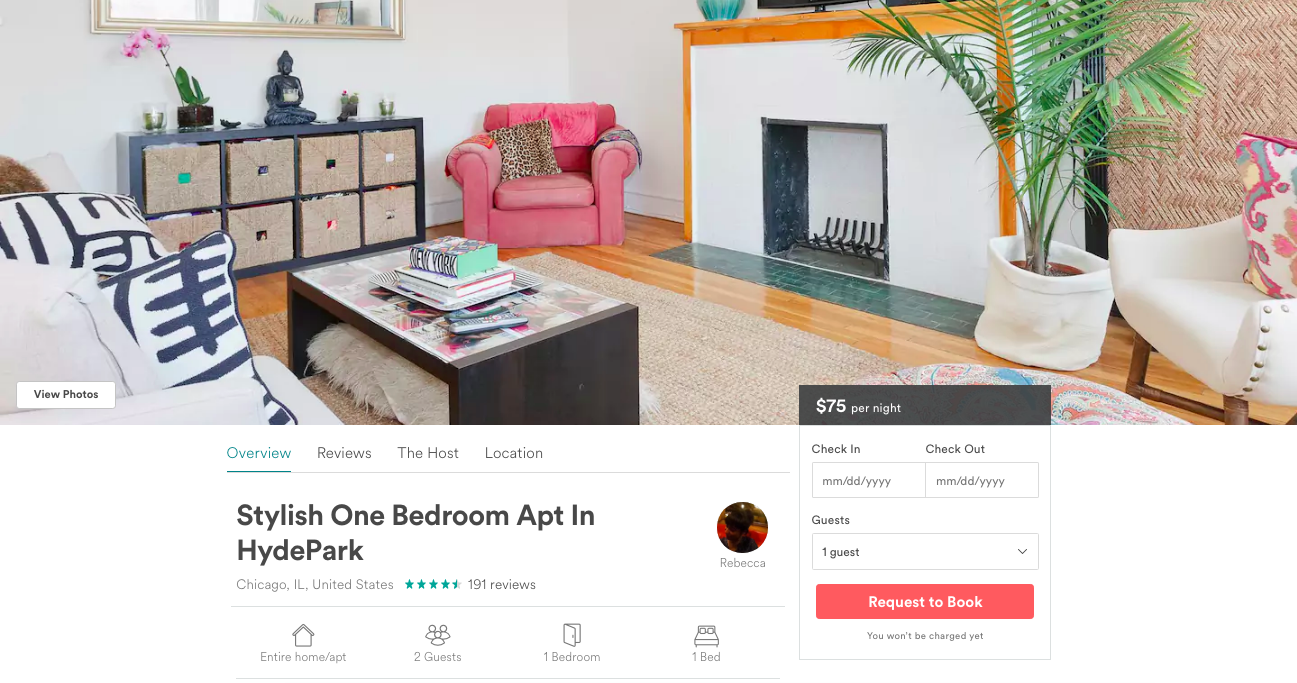
\includegraphics[width=.8\textwidth]{figures/sample1-cover}
	\caption{Sample listing page}
	\label{fig:listing}
\end{figure}

\begin{figure}[!ht]\centering
	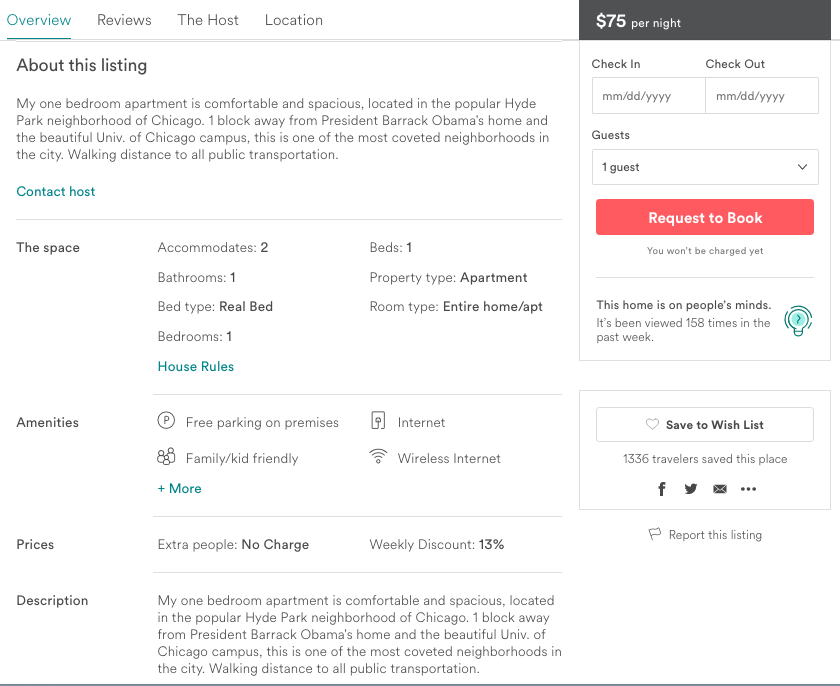
\includegraphics[width=.8\textwidth]{figures/sample2-property}
	\caption{Listing information}
	\label{fig:property}
\end{figure}

\begin{figure}[!ht]\centering
\includegraphics[width=.8\textwidth]{figures/sample3-reviews}
\caption{Review information}
	\label{fig:reviewinfo}
\end{figure}

\begin{figure}\centering
\includegraphics[width=.9\textwidth]{figures/sample4-host}
\caption{Host information}
	\label{fig:host}
\end{figure}

\begin{figure}\centering
\includegraphics[width=.8\textwidth]{figures/sample5-location}
\caption{Location information}
	\label{fig:location}
\end{figure}

\begin{figure}\centering
\includegraphics[width=.8\textwidth]{figures/chicago_city_neighborhoods}
\caption[City of Chicago neighborhoods]{City of Chicago neighborhoods, showing level of granularity of neighborhood controls}
	\label{fig:chicago}
\end{figure}



	
	\newpage
	
% Summary Stats by Host Race: Listing Characteristics
\begin{table}[htbp]
\caption{Summary Statistics By Host Race: Listing Characteristics}
\begin{center}%
\small\begin{tabular}{l c | c | c c c c}
& \multicolumn{1}{c}{} & \multicolumn{5}{c}{Regression Sample}
\\
 \cmidrule(r){3-7}
\\
 & \multicolumn{1}{c}{Full data} & \multicolumn{1}{c}{All} & White & Black & Hispanic & Asian
\\
\hline\hline\noalign{\smallskip} 
 \textit{\textit{Outcome Variables}} & & & & & & \\ Log Price & 4.81 & 4.73 & 4.79 & 4.51 & 4.65 & 4.55 \\
 & (0.75) & (0.66) & (0.66) & (0.62) & (0.65) & (0.64) \\
 Log Number of Reviews & 2.20 & 2.16 & 2.18 & 2.14 & 2.16 & 2.04 \\
 & (1.39) & (1.38) & (1.39) & (1.36) & (1.40) & (1.36) \\
 \textit{Covariates} & & & & & & \\ \hline Property Type & & & & & & \\ \hspace{10bp}Apartments/Lofts    & 0.60 & 0.63 & 0.63 & 0.66 & 0.66 & 0.62 \\ \hspace{10bp}Townhouses/Condos   & 0.04 & 0.04 & 0.04 & 0.04 & 0.04 & 0.06 \\ \hspace{10bp}Houses                      & 0.32 & 0.30 & 0.30 & 0.27 & 0.26 & 0.30 \\ \hspace{10bp}Others                              & 0.04 & 0.03 & 0.03 & 0.03 & 0.03 & 0.03 \\Room Type &&&&&& \\ \hspace{10bp}Entire House/Apartment      & 0.58 & 0.55 & 0.58 & 0.43 & 0.51 & 0.42 \\ \hspace{10bp}Private Room                        & 0.38 & 0.42 & 0.39 & 0.50 & 0.44 & 0.53 \\ \hspace{10bp}Shared Room                         & 0.04 & 0.04 & 0.03 & 0.07 & 0.05 & 0.05 \\ Max Num. Guests & 3.44 & 3.15 & 3.24 & 2.94 & 3.06 & 2.84 \\
 & (2.41) & (2.13) & (2.15) & (2.06) & (2.15) & (2.00) \\
 Bedrooms & 1.34 & 1.26 & 1.28 & 1.19 & 1.21 & 1.18 \\
 & (0.92) & (0.80) & (0.83) & (0.69) & (0.78) & (0.72) \\
 Bathrooms & 1.30 & 1.23 & 1.24 & 1.19 & 1.21 & 1.19 \\
 & (0.69) & (0.55) & (0.56) & (0.49) & (0.52) & (0.53) \\
 Beds & 1.82 & 1.67 & 1.69 & 1.60 & 1.68 & 1.57 \\
 & (1.41) & (1.21) & (1.19) & (1.15) & (1.51) & (1.18) \\
 Cleaning Fee & 48.95 & 43.70 & 46.06 & 36.20 & 40.35 & 36.45 \\
 & (59.62) & (48.32) & (49.73) & (43.18) & (45.51) & (42.86) \\
 Extra Guests Charge & 13.74 & 13.43 & 13.26 & 15.13 & 13.94 & 12.72 \\
 & (23.65) & (22.67) & (23.00) & (22.71) & (22.48) & (20.36) \\
 Minimum Nights & 3.01 & 3.03 & 3.08 & 2.61 & 2.86 & 3.17 \\
 & (9.21) & (8.79) & (9.39) & (4.35) & (6.55) & (8.67) \\
 Availability (out of 30 days) & 11.54 & 11.04 & 10.64 & 14.19 & 11.24 & 10.79 \\
 & (10.93) & (10.91) & (10.75) & (11.49) & (10.94) & (11.01) \\
 Number of Amenities & 0.81 & 0.79 & 0.80 & 0.75 & 0.79 & 0.75 \\
 & (1.10) & (1.10) & (1.10) & (1.04) & (1.10) & (1.13) \\
 Instantly Bookable? & 0.15 & 0.15 & 0.14 & 0.21 & 0.17 & 0.16 \\
 & (0.36) & (0.36) & (0.34) & (0.41) & (0.38) & (0.37) \\
 Year of first review & 14.86 & 14.86 & 14.83 & 14.89 & 14.90 & 15.03 \\
 & (1.22) & (1.22) & (1.22) & (1.30) & (1.21) & (1.17) \\
 Strict Cancellation Policy & 0.43 & 0.40 & 0.42 & 0.42 & 0.42 & 0.42 \\\hline
Observations & \numprint{69007} & \numprint{45076} & \numprint{32934} & \numprint{4354} & \numprint{2913} & \numprint{4875} 
\\
\hline\hline\noalign{\smallskip} \end{tabular} 
\begin{minipage}{6in}
{\it Note:} The values in the table are means and standard deviations of listing-level data in my full sample. Summary statistics for selected covariates are listed in the table. Categorical variables such as room type do not have standard deviations. Property types are explicitly listed if more than 1.5\% of listings are that type. Strict cancellation policy is the most common out of 4 possible policies:  strict (43\%), flexible (31\%), moderate (25\%) and other (1\%) Year of first review is a proxy for the time on the market - 14.86 indicates that the first review of the mean listing in the full sample occurred in October of 2014.
\end{minipage}
\end{center}
\end{table}

\newpage

% Summary Stats by Host Race: Host Demographics
\begin{table}[htbp]
\caption{Summary Statistics By Host Race: Host Demographics}
\begin{center}%
\small\begin{tabular}{l c | c | c c c c}
& \multicolumn{1}{c}{} & \multicolumn{5}{c}{Regression Sample}
\\
 \cmidrule(r){3-7}
\\
 & \multicolumn{1}{c}{Full data} & \multicolumn{1}{c}{All} & White & Black & Hispanic & Asian
\\
\hline\hline\noalign{\smallskip} 
 \textit{Race} &&&&&& \\
 \hspace{10bp}White & 0.64 & 0.73 &  1.00 & 0.00 &  0.00 & 0.00 \\  \hspace{10bp}Black & 0.07 & 0.10 &  0.00 & 1.00 &  0.00 & 0.00 \\  \hspace{10bp}Hispanic & 0.05 & 0.06 &  0.00 & 0.00 &  1.00 & 0.00 \\  \hspace{10bp}Asian & 0.09 & 0.11 &  0.00 & 0.00 &  0.00 & 1.00 \\  \hspace{10bp}Unknown & 0.15 & {0.00} & {0.00} &  {0.00}  & {0.00}  & {0.00} \\  \textit{Sex} &&&&&& \\
 \hspace{10bp}Male & 0.31 & 0.45 &  0.45 & 0.40 &  0.50 & 0.44 \\  \hspace{10bp}Female & 0.38 & 0.55 &  0.55 & 0.60 &  0.50 & 0.56 \\  \hspace{10bp}Unknown & 0.31 & {0.00} & {0.00} &  {0.00}  & {0.00}  & {0.00} \\  \textit{Age} &&&&&& \\
 \hspace{10bp}Young ($<30$) & 0.43 & 0.51 &  0.49 & 0.54 &  0.52 & 0.61 \\  \hspace{10bp}Middle-aged & 0.42 & 0.46 &  0.48 & 0.45 &  0.47 & 0.38 \\  \hspace{10bp}Old ($>65$) & 0.02 & 0.02 &  0.03 & 0.00 &  0.01 & 0.01 \\  \hspace{10bp}Unknown & 0.13 & {0.00} & {0.00} &  {0.00}  & {0.00}  & {0.00} \\ \hline
Observations & \numprint{69000} & \numprint{45076} & \numprint{32934} & \numprint{4354} & \numprint{2913} & \numprint{4875} 
\\
\hline\hline\noalign{\smallskip} \end{tabular} 
\begin{minipage}{6in}
\label{table:host_demographics}
{\it Note:} The values in the table are summaries of host demographics in the host-level data. Column 1 is the summary statistics for the full, unrestricted data set across 7 cities. Columns 2 - 6 are the restricted data used in the analysis. Column 2 is the full regression sample, and columns 3 - 6 break down the regression sample by host race. The “Unknown” category was dropped from the regression and is therefore zero throughout columns 2 - 6. White refers only to Non-Hispanic Whites.\end{minipage}
\end{center}
\end{table}

\newpage

% Summary Stats by Host Race: Host Characteristics
\begin{table}[htbp]
\caption{Summary Statistics By Host Race: Host Characteristics}
\begin{center}%
\small\begin{tabular}{l c | c | c c c c}
& \multicolumn{1}{c}{} & \multicolumn{5}{c}{Regression Sample}
\\
 \cmidrule(r){3-7}
\\
 & \multicolumn{1}{c}{Full data} & \multicolumn{1}{c}{All} & White & Black & Hispanic & Asian
\\
\hline\hline\noalign{\smallskip} 
 \textit{\textit{Outcome Variables}} & & & & & & \\ Host Listings Count & 6.38 & 2.23 & 2.16 & 2.38 & 2.49 & 2.44 \\
 & (36.54) & (2.59) & (2.50) & (2.83) & (3.03) & (2.61) \\
 \textit{Covariates} & & & & & & \\ \hline Review scores rating & 93.56 & 93.68 & 94.18 & 91.91 & 92.80 & 92.26 \\
 & (8.13) & (7.90) & (7.33) & (9.44) & (8.71) & (9.27) \\
 Host is a Superhost & 0.13 & 0.13 & 0.14 & 0.09 & 0.11 & 0.10 \\
 & (0.34) & (0.33) & (0.34) & (0.28) & (0.31) & (0.30) \\
 Response rate & 0.77 & 0.76 & 0.76 & 0.78 & 0.76 & 0.74 \\
 & (0.38) & (0.39) & (0.39) & (0.37) & (0.39) & (0.40) \\
 Acceptance rate & 0.47 & 0.45 & 0.46 & 0.35 & 0.49 & 0.44 \\
 & (0.46) & (0.46) & (0.46) & (0.45) & (0.47) & (0.47) \\
 Polarity of Summary & 0.30 & 0.30 & 0.30 & 0.29 & 0.30 & 0.29 \\
 & (0.17) & (0.17) & (0.17) & (0.16) & (0.17) & (0.17) \\
 Subjectivity of Summary & 0.53 & 0.54 & 0.54 & 0.53 & 0.54 & 0.53 \\
 & (0.15) & (0.15) & (0.15) & (0.15) & (0.15) & (0.15) \\
 Host's Identity Verified? & 0.70 & 0.70 & 0.71 & 0.66 & 0.68 & 0.69 \\
 & (0.46) & (0.46) & (0.45) & (0.47) & (0.47) & (0.46) \\
 Guest Pic Required? & 0.04 & 0.04 & 0.04 & 0.06 & 0.04 & 0.04 \\
 & (0.19) & (0.19) & (0.19) & (0.23) & (0.19) & (0.19) \\
 Guest Phone Required? & 0.05 & 0.05 & 0.05 & 0.06 & 0.04 & 0.04 \\
 & (0.22) & (0.21) & (0.21) & (0.24) & (0.20) & (0.20) \\
 Response time $<$ 1 hour & 0.41 & 0.40 & 0.39 & 0.44 & 0.41 & 0.41 \\\hline
Observations & \numprint{69010} & \numprint{45076} & \numprint{32934} & \numprint{4354} & \numprint{2913} & \numprint{4875}
\\
\hline\hline\noalign{\smallskip} \end{tabular} 
\begin{minipage}{6in}
\label{table:host_summary}
{\it Note:} The values in the table are means and standard deviations of host-level data in the full sample. Summary statistics for selected covariates are listed in the table. Categorical variables such as response time do not have standard deviations. Statistics for only the most frequent response time (\say{within an hour}) are included. White refers only to non-Hispanic whites. Polarity of \say{Summary} and Subjectivity of \say{Summary} refer to the scores from a natural language processing algorithm that measures the sentiment and objectivity of that field. These two measures were also calculated for the description, space, neighborhood overview, notes, and transit fields, but were not included in the table for the sake of clarity and because they follow a similar pattern as the \say{Summary} field.
\end{minipage}
\end{center}
\end{table}

\newpage

% Summary Stats by Race: Reviewer Characteristics
\begin{table}[htbp]
\caption{Summary Statistics By Race: Reviewer Characteristics}
\begin{center}%
\small\begin{tabular}{l c | c | c c c c}
& \multicolumn{1}{c}{} & \multicolumn{5}{c}{Reviewer Race in Chicago data} 
\\
 \cmidrule(r){3-7}
\\
 & \multicolumn{1}{c}{Full data} & \multicolumn{1}{c}{All} & White & Black & Hispanic & Asian
\\
\hline\hline\noalign{\smallskip} 
 Reviewer Race  & 1.00 & 1.00 & 0.66 & 0.03 & 0.04 & 0.11 \\\\
 Host race & & & & & & \\ \hspace{10bp}White &     0.73 & 0.83 & 0.84 & 0.70 & 0.75 & 0.75 \\ \hspace{10bp}Black &     0.06 & 0.06& 0.05 & 0.17 & 0.07 & 0.06 \\ \hspace{10bp}Hispanic &  0.04 & 0.05& 0.05 & 0.06 & 0.10 & 0.08 \\ \hspace{10bp}Asian &     0.05 & 0.05& 0.05 & 0.08 & 0.08 & 0.11 \\ \hspace{10bp}Unknown &   0.12 & 0.00& 0.00 & 0.00 & 0.00 & 0.00 \\\\
 Review Sentiment & 0.51 & 0.51 & 0.51 & 0.50 & 0.47 & 0.53 \\
 & (0.26) & (0.26) & (0.25) & (0.23) & (0.30) & (0.25) \\
\\
 Listing Sentiment & 0.51 & 0.51 & 0.51 & 0.50 & 0.50 & 0.51 \\
 & (0.07) & (0.07) & (0.07) & (0.07) & (0.07) & (0.09) \\
\\
\hline
Observations & \numprint{17050} &  \numprint{10573} & \numprint{6929} & \numprint{319} & \numprint{402} & \numprint{1153}
\\
\hline\hline\noalign{\smallskip} \end{tabular} 
\begin{minipage}{6in}
\label{table:reviewer_demographics}
{\it Note:} The values in this table are means and standard deviations of reviewer-level data who left reviews for a randomly chosen set of hosts in Chicago. Column 1 presents the means for the full reviewer data. Column 2 presents the means of the sample used in Table \ref{table:sentiment}. Columns 3 - 6 partition Column 2 by reviewer race. Row 1, \say{Reviewer race} indicates the proportion of the different reviewer races in the data coded. Row 2, \say{Host race} indicates the marginal probability of a host race given a reviewer race. The review sentiment is the sentiment of each review, the listing sentiment is the average sentiment per listing. Observations in Columns 2 - 5 do not add up to 17,050 because multiracial or unidentifiable reviewer pictures are excluded. White refers only to non-Hispanic Whites.
\end{minipage}
\end{center}
\end{table}

\newpage

% Price
\begin{table}[htbp]\centering
	\def\sym#1{\ifmmode^{#1}\else\(^{#1}\)\fi}
	\caption{Main result: Estimates of effect of host’s race and gender on price}
	\begin{tabular}{l*{5}{c}}
		\hline\hline
		                    &\multicolumn{1}{c}{(1)}&\multicolumn{1}{c}{(2)}&\multicolumn{1}{c}{(3)}&\multicolumn{1}{c}{(4)}\\
                    &\multicolumn{1}{c}{Model 1}&\multicolumn{1}{c}{Model 2}&\multicolumn{1}{c}{Model 3}&\multicolumn{1}{c}{Model 4}\\
\hline
White Female        &     -0.0236\sym{*}  &     -0.0138         &     0.00201         &     0.00298         \\
                    &    (0.0106)         &   (0.00854)         &   (0.00496)         &   (0.00484)         \\
[1em]
Black Male          &      -0.276\sym{***}&     -0.0828\sym{**} &     -0.0360\sym{**} &     -0.0328\sym{**} \\
                    &    (0.0315)         &    (0.0259)         &    (0.0123)         &    (0.0123)         \\
[1em]
Black Female        &      -0.299\sym{***}&     -0.0586\sym{**} &     -0.0196         &     -0.0167         \\
                    &    (0.0296)         &    (0.0188)         &    (0.0102)         &   (0.00996)         \\
[1em]
Hispanic Male       &      -0.153\sym{***}&     -0.0521\sym{**} &     -0.0233\sym{*}  &     -0.0200         \\
                    &    (0.0259)         &    (0.0191)         &    (0.0113)         &    (0.0113)         \\
[1em]
Hispanic Female     &      -0.150\sym{***}&     -0.0653\sym{**} &     -0.0196         &     -0.0202         \\
                    &    (0.0280)         &    (0.0202)         &    (0.0115)         &    (0.0114)         \\
[1em]
Asian Male          &      -0.221\sym{***}&     -0.0987\sym{***}&     -0.0425\sym{**} &     -0.0446\sym{***}\\
                    &    (0.0336)         &    (0.0225)         &    (0.0134)         &    (0.0135)         \\
[1em]
Asian Female        &      -0.283\sym{***}&      -0.131\sym{***}&     -0.0409\sym{***}&     -0.0396\sym{***}\\
                    &    (0.0299)         &    (0.0161)         &   (0.00874)         &   (0.00893)         \\
[1em]
Constant            &       4.802\sym{***}&       4.979\sym{***}&       3.891\sym{***}&       4.003\sym{***}\\
                    &    (0.0300)         &     (0.398)         &     (0.343)         &     (0.344)         \\
\hline
Location Controls   &                     &         Yes         &         Yes         &         Yes         \\
Property Controls   &                     &                     &         Yes         &         Yes         \\
Host Controls       &                     &                     &                     &         Yes         \\
\hline \vspace{-1.25em}&                     &                     &                     &                     \\
Observations        &       45073         &       45073         &       45073         &       45073         \\
Adjusted R2         &      0.0263         &       0.246         &       0.716         &       0.720         \\

		\hline\hline
		\multicolumn{5}{l}{\footnotesize Standard errors in parentheses}\\
		\multicolumn{5}{l}{\footnotesize \sym{*} \(p<0.05\), \sym{**} \(p<0.01\), \sym{***} \(p<0.001\)}\\
	\end{tabular}	
\label{table:price}
	\begin{tablenotes}
		
		\item {\it Note:} This table presents the impact of host race on the price of a listing. The dependent variable is the log price. The omitted category is White males. The unit of observation is a listing. The sample is the sample of listings across 7 US cities. Model 1 is the baseline effect of host demographics on price. Model 2 controls for listing location to the neighborhood level and demographic and economic health characteristics on the zipcode-level. Model 3 adds listing characteristics such as the property type and size. Model 4 adds host characteristics such as response and acceptance rates and measures of host effort.  
	\end{tablenotes}
\end{table}



% ALL MEASURES of QD
\begin{table}[htbp]\centering
	\def\sym#1{\ifmmode^{#1}\else\(^{#1}\)\fi}
	\caption{Effect of host’s race on two proxies of quantity demanded}
	\begin{tabular}{l*{2}{c}}
		\hline\hline
		\input{code/tables/tex_output/individual_tables/quantity_demanded}
		\hline\hline
		\multicolumn{2}{l}{\footnotesize Standard errors in parentheses}\\
		\multicolumn{2}{l}{\footnotesize \sym{*} \(p<0.05\), \sym{**} \(p<0.01\), \sym{***} \(p<0.001\)}\\
	\end{tabular}
\label{table:quantity_demanded}
	\begin{tablenotes}
		\item {\it Note:} This table presents the effect of host race on two proxies of quantity demanded: a listing's availability out of 30 days and the log of its number of reviews. When a listing is booked, this availability metric is updated on the Airbnb website to reflect that booking. Therefore, the availability metric actually represents the number of days out of the total available days that listings were vacant. I control for the specification in Table \ref{table:price}, Model 4.
	\end{tablenotes}
\end{table}


% Robustness city NEW, with interaction
\begin{table}[htbp]\centering
	\def\sym#1{\ifmmode^{#1}\else\(^{#1}\)\fi}
	\caption{Robustness City}
	\begin{tabular}{l*{7}{c}}
		\hline\hline
		\input{code/tables/tex_output/individual_tables/price_by_city}
		\hline\hline
		\multicolumn{8}{l}{\footnotesize Standard errors in parentheses}\\
		\multicolumn{8}{l}{\footnotesize \sym{*} \(p<0.05\), \sym{**} \(p<0.01\), \sym{***} \(p<0.001\)}\\
	\end{tabular}
	\label{table:robustcity}
	\begin{tablenotes}
		
		\item {\it Note:} This table breaks down the effects for the combined data in Table \ref{table:price} across the 7 cities in the sample. Each set of coefficients represents the coefficient on host race, with log price as the outcome variable. I control for my preferred specification throughout. Low number of observations for Black, Hispanic, and Asian hosts contribute to imprecise estimates in smaller cities (New Orleans, Nashville have less than 100 Hispanic and Asian hosts; DC and Austin have less than 200 such hosts). 
	\end{tablenotes}
\end{table}


\begin{landscape}
	% Robustness Listing Characteristics 
	\begin{table}[htbp]\centering
		\def\sym#1{\ifmmode^{#1}\else\(^{#1}\)\fi}
		\caption{NEW: Robustness Listing Characteristics}
		\begin{tabular}{l*{8}{c}}
			\hline\hline
			\input{code/tables/tex_output/individual_tables/price_by_listing_type}
			\hline\hline
			\multicolumn{9}{l}{\footnotesize Standard errors in parentheses}\\
			\multicolumn{9}{l}{\footnotesize \sym{*} \(p<0.05\), \sym{**} \(p<0.01\), \sym{***} \(p<0.001\)}\\
		\end{tabular}
		\label{table:robustlisting}
		\begin{tablenotes}
			\item {\it Note:} This table breaks the effects for the combined data by only high-priced listings versus all prices, listings with greater than 5 reviews, the time on market, and property type. The categories, from left to right, are: listings whose price are above the cutoff price in the original sample, listings of all prices, listings with more than 5 reviews, listings who have have been on the market for no more than 2 years vs. no more than 8 years, and listings of different property types, including apartments (includes apartments and lofts), condos (includes condos and townhouse), and houses. I control for my preferred specification throughout. The outcome variable is the log price of the listing.
		\end{tablenotes}
	\end{table}
\end{landscape}


% Host demographics on review sentiment, by reviewer demographics
\begin{landscape}
	\begin{table}[htbp]\centering
		\def\sym#1{\ifmmode^{#1}\else\(^{#1}\)\fi}
		\caption{Estimates of effect of host demographics on review sentiment, by reviewer demographics}
		\begin{tabular}{l *{8}{c}}
			\hline\hline
			&\multicolumn{8}{c}{Reviewers} \\
			\cmidrule(r){2-9}\\
			                    &\multicolumn{1}{c}{(1)}&\multicolumn{1}{c}{(2)}&\multicolumn{1}{c}{(3)}&\multicolumn{1}{c}{(4)}&\multicolumn{1}{c}{(5)}&\multicolumn{1}{c}{(6)}&\multicolumn{1}{c}{(7)}&\multicolumn{1}{c}{(8)}\\
                    &\multicolumn{1}{c}{White M}&\multicolumn{1}{c}{White F}&\multicolumn{1}{c}{Black M}&\multicolumn{1}{c}{Black F}&\multicolumn{1}{c}{Hispanic M}&\multicolumn{1}{c}{Hispanic F}&\multicolumn{1}{c}{Asian M}&\multicolumn{1}{c}{Asian F}\\
\hline
White Female        &     -0.0780         &      0.0371         &     -0.0475         &       2.352\sym{***}&      -0.326         &      -0.912\sym{***}&       0.139         &      0.0114         \\
                    &    (0.0733)         &    (0.0471)         &    (0.0774)         &     (0.435)         &     (0.276)         &  (2.58e-13)         &     (0.356)         &     (0.209)         \\
Black Male          &      -0.175         &      -0.164         &     -0.0635         &       1.419         &      -0.172         &       1.230\sym{***}&       0.932         &      -3.941\sym{*}  \\
                    &     (0.205)         &     (0.296)         &     (0.369)         &     (0.822)         &     (1.052)         &  (1.28e-12)         &     (0.823)         &     (1.613)         \\
Black Female        &     -0.0793         &      0.0249         &      0.0551         &      -5.562\sym{***}&      0.0769         &       0.350\sym{***}&       0.379         &      0.0576         \\
                    &     (0.177)         &     (0.110)         &     (0.134)         &     (1.034)         &     (0.665)         &  (1.54e-12)         &     (0.533)         &     (0.660)         \\
Hispanic Male       &     -0.0350         &      0.0716         &      -0.337\sym{*}  &      -0.756         &       0.803         &       0.521\sym{***}&      -0.630         &      -0.572         \\
                    &     (0.104)         &     (0.135)         &     (0.131)         &     (0.545)         &     (0.618)         &  (1.63e-14)         &     (0.641)         &     (1.059)         \\
Hispanic Female     &      0.0119         &     -0.0751         &      0.0352         &       9.364\sym{***}&      -1.363         &      -1.933\sym{***}&      -1.098         &       1.345\sym{*}  \\
                    &     (0.360)         &    (0.0722)         &     (0.226)         &     (1.293)         &     (2.832)         &  (1.54e-12)         &     (0.899)         &     (0.497)         \\
Asian Male          &      -0.329         &      -0.248         &       0.211         &       9.200\sym{***}&       0.306         &       0.853\sym{***}&    -0.00444         &      -1.307         \\
                    &     (0.240)         &     (0.169)         &     (0.261)         &     (1.510)         &     (0.799)         &  (1.03e-12)         &     (1.091)         &     (1.864)         \\
Asian Female        &      -0.282         &      -0.269         &      -0.388         &       13.96\sym{***}&       0.985         &      -0.960\sym{***}&      -0.986         &      -0.725         \\
                    &     (0.167)         &     (0.147)         &     (0.228)         &     (1.832)         &     (0.609)         &  (1.80e-12)         &     (0.893)         &     (0.546)         \\
\hline
Location Controls   &         Yes         &         Yes         &         Yes         &         Yes         &         Yes         &         Yes         &         Yes         &         Yes         \\
Property Controls   &         Yes         &         Yes         &         Yes         &         Yes         &         Yes         &         Yes         &         Yes         &         Yes         \\
Host Controls       &         Yes         &         Yes         &         Yes         &         Yes         &         Yes         &         Yes         &         Yes         &         Yes         \\
\hline \vspace{-1.25em}&                     &                     &                     &                     &                     &                     &                     &                     \\
Observations        &        2665         &        2527         &        1737         &         121         &         171         &          27         &         198         &         142         \\
Adjusted R2         &      0.0504         &      0.0454         &      0.0657         &       0.826         &       0.622         &       0.970         &       0.500         &       0.685         \\
	
			\hline\hline
			\multicolumn{9}{l}{\footnotesize Standard errors in parentheses}\\
			\multicolumn{9}{l}{\footnotesize \sym{*} \(p<0.05\), \sym{**} \(p<0.01\), \sym{***} \(p<0.001\)}\\
		\end{tabular}
	\label{table:sentiment}
	
		\begin{tablenotes}
			
			\item {\it Note:} This table measures the quality of a review that reviewers leave for hosts in Chicago. The columns are the demographics of the reviewers (male is \say{M}, female is \say{F}), and the rows are the demographics of the host. The outcome variable is the sentiment of the review. Each coefficient is the standardized sentiment of a review. Review sentiment measures how positive or negative the review is. Reviews that are numerically positive are of positive sentiment and numerically negative are negative sentiment, relative to the mean sentiment score for each host type. The unit of observation is a single review. The data is a subsample of the Chicago hosts and their reviewers. I control for my preferred specification throughout. 
			
		\end{tablenotes}
		
	\end{table}
\end{landscape}












\newpage

\section*{Appendix Tables}

% Edelman & Luca
\begin{table}[htbp]\centering
	\def\sym#1{\ifmmode^{#1}\else\(^{#1}\)\fi}
	
	\caption{Robustness check with controls from Edelman \& Luca (2014)}
	\begin{tabular}{l*{1}{c}}
		\hline\hline
		                    &\multicolumn{1}{c}{(1)}\\
                    &\multicolumn{1}{c}{Price per night}\\
\hline
Black               &      -0.117\sym{***}\\
                    &    (0.0107)         \\
Accommodates        &      0.0684\sym{***}\\
                    &   (0.00288)         \\
Bedrooms            &       0.129\sym{***}\\
                    &   (0.00724)         \\
Review Scores Location&      -0.488\sym{***}\\
                    &    (0.0434)         \\
Review Scores Location Squared&      0.0363\sym{***}\\
                    &   (0.00249)         \\
Review Scores Checkin&   -0.000735         \\
                    &   (0.00683)         \\
Review Scores Communication&    -0.00366         \\
                    &   (0.00718)         \\
Review Scores Cleanliness&      0.0230\sym{***}\\
                    &   (0.00417)         \\
Review Scores Accuracy&     -0.0186\sym{**} \\
                    &   (0.00574)         \\
Host's Identity Verified?&      0.0233\sym{**} \\
                    &   (0.00801)         \\
Private room        &      -0.627\sym{***}\\
                    &   (0.00826)         \\
Shared room         &      -1.123\sym{***}\\
                    &    (0.0183)         \\
\hline
Location Controls   &         Yes         \\
Property Controls   &         Yes         \\
Host Controls       &         Yes         \\
\hline \vspace{-1.25em}&                     \\
Observations        &       11999         \\
Adjusted R2         &       0.619         \\
 
		\hline\hline
		\multicolumn{2}{l}{\footnotesize Standard errors in parentheses}\\
		\multicolumn{2}{l}{\footnotesize \sym{*} \(p<0.05\), \sym{**} \(p<0.01\), \sym{***} \(p<0.001\)}\\
	\end{tabular}
	\label{table:edelman}
	\begin{tablenotes}
		\item {\it Note:} This table presents the effect on log price of controlling for Edelman \& Luca's (2014) full specification using my NYC data. The omitted category for race is White hosts. The omitted category for room type is Entire Apartment. I could not control for host social media accounts as a proxy for host reliability like Edelman \& Luca did, because Airbnb no longer provides this information. Instead, I controlled for ``host verified", a dummy for whether Airbnb has the host's phone number and email. I was not able to control for ``picture quality" either, but picture quality did not significantly influence price in Edelman \& Luca's regression.
	\end{tablenotes}
\end{table}


% Robustness host listings count
\begin{table}[htbp]\centering
	\def\sym#1{\ifmmode^{#1}\else\(^{#1}\)\fi}
	\caption{Estimates of effect of host listings count on price}
	\begin{tabular}{l*{6}{c}}
		\hline\hline
		\input{code/tables/tex_output/individual_tables/robustness_listings_count}
		\hline\hline
		\multicolumn{5}{l}{\footnotesize Standard errors in parentheses}\\
		\multicolumn{5}{l}{\footnotesize \sym{*} \(p<0.05\), \sym{**} \(p<0.01\), \sym{***} \(p<0.001\)}\\
	\end{tabular}
	\label{table:robustness_listings_count}
	\begin{tablenotes}

		\item {\it Note:} Insert note here
	\end{tablenotes}
\end{table}


% Price, no interaction
\begin{table}[htbp]\centering
	\def\sym#1{\ifmmode^{#1}\else\(^{#1}\)\fi}
	\caption{Main result: Estimates of effect of host’s race and gender on price [Without interaction]}
	\begin{tabular}{l*{5}{c}}
		\hline\hline
		\input{code/tables/tex_output/individual_tables/price_no_int}
		\hline\hline
		\multicolumn{5}{l}{\footnotesize Standard errors in parentheses}\\
		\multicolumn{5}{l}{\footnotesize \sym{*} \(p<0.05\), \sym{**} \(p<0.01\), \sym{***} \(p<0.001\)}\\
	\end{tabular}
	\label{table:price_no_int}
	\begin{tablenotes}
		
		\item {\it Note:} The dependent variable is the log price of the listing. The omitted category for host race and gender is White hosts. The unit of observation is a listing. The sample is the sample of listings across 7 US cities. Model 1 is the baseline effect of host demographics on price. Model 2 controls for listing location to the neighborhood level and demographic and economic health characteristics on the zipcode-level. Model 3 adds listing characteristics such as the property type and size. Model 4 adds host characteristics such as response and acceptance rates and measures of host effort.  
	\end{tablenotes}
\end{table}


% Yearly revenue
\begin{table}[htbp]\centering
	\def\sym#1{\ifmmode^{#1}\else\(^{#1}\)\fi}
	\caption{Estimates of effect of host's race and gender on yearly revenue}
	\begin{tabular}{l*{4}{c}}
		\hline\hline
		                    &\multicolumn{1}{c}{(1)}&\multicolumn{1}{c}{(2)}&\multicolumn{1}{c}{(3)}&\multicolumn{1}{c}{(4)}\\
                    &\multicolumn{1}{c}{Model 1}&\multicolumn{1}{c}{Model 2}&\multicolumn{1}{c}{Model 3}&\multicolumn{1}{c}{Model 4}\\
\hline
White Female        &      -199.0\sym{***}&      -156.5\sym{***}&      -151.9\sym{***}&       92.25         \\
                    &     (48.54)         &     (46.80)         &     (39.72)         &     (296.6)         \\
[1em]
Black Male          &      -655.0\sym{***}&      -329.5\sym{***}&      -261.8\sym{***}&       290.8         \\
                    &     (98.27)         &     (96.15)         &     (59.77)         &     (608.6)         \\
[1em]
Black Female        &      -814.7\sym{***}&      -365.0\sym{***}&      -319.5\sym{***}&       575.1         \\
                    &     (96.68)         &     (78.69)         &     (51.94)         &     (763.7)         \\
[1em]
Hispanic Male       &      -209.0         &      -44.57         &      -25.43         &      -328.9         \\
                    &     (112.5)         &     (97.48)         &     (88.24)         &     (766.3)         \\
[1em]
Hispanic Female     &      -280.8\sym{*}  &      -79.57         &      -118.8         &      3219.4         \\
                    &     (140.1)         &     (120.6)         &     (108.1)         &    (3499.2)         \\
[1em]
Asian Male          &      -360.5\sym{**} &      -95.81         &      -15.85         &       180.6         \\
                    &     (129.4)         &     (115.4)         &     (88.42)         &    (1378.4)         \\
[1em]
Asian Female        &      -676.6\sym{***}&      -329.2\sym{***}&      -183.7\sym{**} &     -1684.3         \\
                    &     (98.12)         &     (74.92)         &     (62.31)         &     (866.0)         \\
[1em]
Constant            &      2301.2\sym{***}&      3975.9\sym{***}&      1097.5\sym{***}&     -6935.1         \\
                    &     (109.2)         &     (36.27)         &     (169.1)         &    (4465.5)         \\
\hline
Location Controls   &                     &         Yes         &         Yes         &         Yes         \\
Property Controls   &                     &                     &         Yes         &         Yes         \\
Host Controls       &                     &                     &                     &         Yes         \\
\hline \vspace{-1.25em}&                     &                     &                     &                     \\
Observations        &       45072         &       45072         &       45072         &         356         \\
Adjusted R2         &     0.00628         &      0.0959         &       0.361         &       0.538         \\

		\hline\hline
		\multicolumn{5}{l}{\footnotesize Standard errors in parentheses}\\
		\multicolumn{5}{l}{\footnotesize \sym{*} \(p<0.05\), \sym{**} \(p<0.01\), \sym{***} \(p<0.001\)}\\
	\end{tabular}
	\label{revenue}
	\begin{tablenotes}
		\item {\it Note:} The dependent variable is a measure of yearly host revenue, as measured by for each listing. The omitted category for race is White males, so all coefficients are relative to that group. The unit of observation is an Airbnb listing, so hosts who have multiple listings are treated separately each time. The sample is the sample of listings across 7 US cities. The specification is the same as Table \ref{table:price}.
	\end{tablenotes}
\end{table}


















\begin{comment}

%  Number of reviews
\begin{table}[htbp]\centering
\def\sym#1{\ifmmode^{#1}\else\(^{#1}\)\fi}
\caption{Estimates of effect of host’s race and gender on number of reviews}
\begin{tabular}{l*{4}{c}}
\hline\hline
                    &\multicolumn{1}{c}{(1)}&\multicolumn{1}{c}{(2)}&\multicolumn{1}{c}{(3)}&\multicolumn{1}{c}{(4)}\\
                    &\multicolumn{1}{c}{Model 1}&\multicolumn{1}{c}{Model 2}&\multicolumn{1}{c}{Model 3}&\multicolumn{1}{c}{Model 4}\\
\hline
White Female        &     -0.0646\sym{**} &     -0.0489\sym{*}  &     -0.0651\sym{***}&     -0.0516\sym{**} \\
                    &    (0.0246)         &    (0.0232)         &    (0.0164)         &    (0.0162)         \\
[1em]
Black Male          &     -0.0618         &     -0.0528         &     -0.0867\sym{**} &     -0.0619         \\
                    &    (0.0636)         &    (0.0542)         &    (0.0334)         &    (0.0321)         \\
[1em]
Black Female        &     -0.0626         &     -0.0633         &      -0.144\sym{***}&      -0.104\sym{***}\\
                    &    (0.0634)         &    (0.0575)         &    (0.0301)         &    (0.0271)         \\
[1em]
Hispanic Male       &     -0.0920         &     -0.0398         &     -0.0567         &     -0.0534         \\
                    &    (0.0530)         &    (0.0503)         &    (0.0353)         &    (0.0315)         \\
[1em]
Hispanic Female     &    0.000356         &      0.0468         &     -0.0277         &      0.0191         \\
                    &    (0.0589)         &    (0.0565)         &    (0.0377)         &    (0.0364)         \\
[1em]
Asian Male          &     -0.0872         &      0.0114         &     -0.0145         &     -0.0147         \\
                    &    (0.0542)         &    (0.0468)         &    (0.0374)         &    (0.0319)         \\
[1em]
Asian Female        &      -0.182\sym{***}&     -0.0662         &     -0.0998\sym{***}&     -0.0529\sym{*}  \\
                    &    (0.0523)         &    (0.0412)         &    (0.0278)         &    (0.0251)         \\
[1em]
Constant            &       1.251\sym{***}&       1.591\sym{**} &       4.876\sym{***}&       3.910\sym{***}\\
                    &     (0.231)         &     (0.558)         &     (0.531)         &     (0.416)         \\
\hline
Location Controls   &                     &         Yes         &         Yes         &         Yes         \\
Property Controls   &                     &                     &         Yes         &         Yes         \\
Host Controls       &                     &                     &                     &         Yes         \\
\hline \vspace{-1.25em}&                     &                     &                     &                     \\
Observations        &       35734         &       35734         &       35734         &       35734         \\
Adjusted R2         &      0.0102         &      0.0742         &       0.455         &       0.559         \\

\hline\hline
\multicolumn{5}{l}{\footnotesize Standard errors in parentheses}\\
\multicolumn{5}{l}{\footnotesize \sym{*} \(p<0.05\), \sym{**} \(p<0.01\), \sym{***} \(p<0.001\)}\\
\end{tabular}
\label{table:num_reviews}

\begin{tablenotes}
\item {\it Note:} The dependent variable is the log number of reviews of the listing. The omitted category for race is White males. The unit of observation is an Airbnb listing, so hosts who have multiple listings are treated separately each time. The sample is the sample of listings across 7 US cities. The specification is the same as Table \ref{table:price}.	
\end{tablenotes}
\end{table}


% GARBAGE Chicago price, ML sentiment controls
\begin{table}[htbp]\centering
\def\sym#1{\ifmmode^{#1}\else\(^{#1}\)\fi}
\caption{Main result: Estimates of effect of Chicago host’s race and gender on price, ML sentiment controls}
\begin{tabular}{l*{5}{c}}
\hline\hline
\input{code/tables/tex_output/individual_tables/chicago_price_sentiment}
\hline\hline
\multicolumn{5}{l}{\footnotesize Standard errors in parentheses}\\
\multicolumn{5}{l}{\footnotesize \sym{*} \(p<0.05\), \sym{**} \(p<0.01\), \sym{***} \(p<0.001\)}\\
\end{tabular}	
\label{table:chiprice}
\begin{tablenotes}

\item {\it Note:} This table presents the impact of host race on the price of a listing. The dependent variable is the log price. The omitted category is White males. The unit of observation is a listing. The sample is the sample of listings in Chicago. Model 1 is the baseline effect of host demographics on price. Model 2 controls for listing location to the neighborhood level and demographic and economic health characteristics on the zipcode-level. Model 3 adds listing characteristics such as the property type and size. Model 4 adds host characteristics such as response and acceptance rates and measures of host effort.  
\end{tablenotes}
\end{table}


% OLD Robustness City
\begin{table}[htbp]\centering
\def\sym#1{\ifmmode^{#1}\else\(^{#1}\)\fi}
\caption{Robustness City}
\begin{tabular}{l*{7}{c}}
\hline\hline
                    &\multicolumn{1}{c}{(1)}&\multicolumn{1}{c}{(2)}&\multicolumn{1}{c}{(3)}&\multicolumn{1}{c}{(4)}&\multicolumn{1}{c}{(5)}&\multicolumn{1}{c}{(6)}&\multicolumn{1}{c}{(7)}\\
                    &\multicolumn{1}{c}{LA}&\multicolumn{1}{c}{NYC}&\multicolumn{1}{c}{Austin}&\multicolumn{1}{c}{Chicago}&\multicolumn{1}{c}{New Orleans}&\multicolumn{1}{c}{DC}&\multicolumn{1}{c}{Nashville}\\
\hline
Female              &    -0.00241         &     0.00823         &      0.0152         &     -0.0230         &      0.0259         &      0.0337\sym{**} &      0.0194         \\
                    &   (0.00636)         &   (0.00618)         &    (0.0153)         &    (0.0162)         &    (0.0189)         &    (0.0122)         &    (0.0169)         \\
[1em]
Black               &     -0.0290\sym{*}  &    -0.00470         &     -0.0770         &     -0.0283         &     -0.0588         &     -0.0628         &     -0.0612         \\
                    &    (0.0118)         &   (0.00944)         &    (0.0677)         &    (0.0307)         &    (0.0451)         &    (0.0337)         &    (0.0496)         \\
[1em]
Hispanic            &     -0.0315\sym{**} &     -0.0165         &      0.0220         &     -0.0478\sym{*}  &     0.00187         &    -0.00452         &      -0.144\sym{*}  \\
                    &    (0.0100)         &    (0.0138)         &    (0.0261)         &    (0.0205)         &    (0.0469)         &    (0.0250)         &    (0.0581)         \\
[1em]
Asian               &     -0.0310\sym{**} &     -0.0357\sym{*}  &      -0.104\sym{*}  &      -0.104\sym{**} &     -0.0161         &     -0.0550\sym{**} &     -0.0645         \\
                    &    (0.0108)         &    (0.0141)         &    (0.0459)         &    (0.0315)         &    (0.0618)         &    (0.0186)         &    (0.0579)         \\
\hline
\textit{Fixed Effects:}&                     &                     &                     &                     &                     &                     &                     \\
Location Controls   &         Yes         &         Yes         &         Yes         &         Yes         &         Yes         &         Yes         &         Yes         \\
Property Controls   &         Yes         &         Yes         &         Yes         &         Yes         &         Yes         &         Yes         &         Yes         \\
Host Controls       &         Yes         &         Yes         &         Yes         &         Yes         &         Yes         &         Yes         &         Yes         \\
\hline \vspace{-1.25em}&                     &                     &                     &                     &                     &                     &                     \\
Observations        &       16824         &       14765         &        3635         &        3255         &        2562         &        2285         &        1747         \\
Adjusted R2         &       0.754         &       0.735         &       0.722         &       0.730         &       0.675         &       0.675         &       0.773         \\

\hline\hline
\multicolumn{8}{l}{\footnotesize Standard errors in parentheses}\\
\multicolumn{8}{l}{\footnotesize \sym{*} \(p<0.05\), \sym{**} \(p<0.01\), \sym{***} \(p<0.001\)}\\
\end{tabular}
\label{table:robustcity_old}

\begin{tablenotes}
\item {\it Note:} This table breaks down the effects for the combined data in Table \ref{table:price} across the 7 cities in the sample. Each set of coefficients represents the coefficient on host race, with log price as the outcome variable. I control for my preferred specification throughout. Low number of observations for Black, Hispanic, and Asian hosts contribute to imprecise estimates in smaller cities (New Orleans, Nashville have less than 100 Hispanic and Asian hosts; DC and Austin have less than 200 such hosts). 
\end{tablenotes}
\end{table}

% OLD Robustness Listing Characteristics
\begin{landscape}
\begin{table}[htbp]\centering
\def\sym#1{\ifmmode^{#1}\else\(^{#1}\)\fi}
\caption{Robustness Listing Characteristics}
\begin{tabular}{l*{9}{c}}
\hline\hline
                    &\multicolumn{1}{c}{(1)}&\multicolumn{1}{c}{(2)}&\multicolumn{1}{c}{(3)}&\multicolumn{1}{c}{(4)}&\multicolumn{1}{c}{(5)}&\multicolumn{1}{c}{(6)}&\multicolumn{1}{c}{(7)}&\multicolumn{1}{c}{(8)}&\multicolumn{1}{c}{(9)}\\
                    &\multicolumn{1}{c}{Low \$ LA}&\multicolumn{1}{c}{High \$ LA}&\multicolumn{1}{c}{Low \$ NY}&\multicolumn{1}{c}{High \$ NY}&\multicolumn{1}{c}{Older Listings}&\multicolumn{1}{c}{Newer Listings}&\multicolumn{1}{c}{Apartments}&\multicolumn{1}{c}{Condos}&\multicolumn{1}{c}{Houses}\\
\hline
Black               &     -0.0278\sym{*}  &     -0.0360         &      0.0154         &     -0.0597\sym{***}&     -0.0337\sym{*}  &     -0.0364\sym{***}&     -0.0246\sym{**} &     0.00348         &     -0.0441\sym{*}  \\
                    &    (0.0127)         &    (0.0302)         &   (0.00952)         &    (0.0156)         &    (0.0156)         &   (0.00901)         &   (0.00902)         &    (0.0407)         &    (0.0179)         \\
[1em]
Hispanic            &     -0.0293\sym{**} &     -0.0491         &     -0.0152         &    -0.00604         &     -0.0349\sym{*}  &     -0.0170         &     -0.0217\sym{*}  &     -0.0331         &     -0.0380\sym{*}  \\
                    &    (0.0104)         &    (0.0291)         &    (0.0190)         &    (0.0150)         &    (0.0153)         &   (0.00970)         &   (0.00925)         &    (0.0441)         &    (0.0170)         \\
[1em]
Asian               &     -0.0301\sym{**} &     -0.0579\sym{*}  &     -0.0370\sym{*}  &     -0.0354\sym{*}  &     -0.0252\sym{*}  &     -0.0408\sym{***}&     -0.0388\sym{***}&     -0.0575         &     -0.0469\sym{**} \\
                    &    (0.0109)         &    (0.0227)         &    (0.0170)         &    (0.0152)         &    (0.0119)         &    (0.0113)         &    (0.0100)         &    (0.0387)         &    (0.0145)         \\
\hline
Location Controls   &         Yes         &         Yes         &         Yes         &         Yes         &         Yes         &         Yes         &         Yes         &         Yes         &         Yes         \\
Property Controls   &         Yes         &         Yes         &         Yes         &         Yes         &         Yes         &         Yes         &         Yes         &         Yes         &         Yes         \\
Host Controls       &         Yes         &         Yes         &         Yes         &         Yes         &         Yes         &         Yes         &         Yes         &         Yes         &         Yes         \\
\hline \vspace{-1.25em}&                     &                     &                     &                     &                     &                     &                     &                     &                     \\
Observations        &       13005         &        3819         &        8271         &        6494         &        9846         &       25882         &       28408         &        1854         &       13509         \\
Adjusted R2         &       0.560         &       0.544         &       0.428         &       0.525         &       0.770         &       0.763         &       0.684         &       0.786         &       0.795         \\

\hline\hline
\multicolumn{10}{l}{\footnotesize Standard errors in parentheses}\\
\multicolumn{10}{l}{\footnotesize \sym{*} \(p<0.05\), \sym{**} \(p<0.01\), \sym{***} \(p<0.001\)}\\
\end{tabular}
\label{table:robustlistingold}

\begin{tablenotes}
\item {\it Note:} This table breaks the effects for the combined data by high versus low price, time on market, and property type. The categories, from left to right, are: listings whose log price is below vs. above the mean predicted log price in each city, the price originally dropped, listings who have have been on the market for no more than 2 years vs. no more than 8 years, and listings of different property types, including apartments (includes apartments and lofts), condos (includes condos and townhouse), and houses. I control for my preferred specification throughout. The outcome variable is the log price of the listing.
\end{tablenotes}
\end{table}
\end{landscape}

\end{comment}


	
	
	\begin{comment}
	
	***************** TRASH SECTION
	
	Options for first sentence of abstract:
	\begin{enumerate}
	\item The extent of discrimination on Airbnb, especially against hosts, remains poorly researched. 
	\item Despite well-publicized efforts by Airbnb to address discrimination on its platform, the discrimination against hosts remains poorly measured by economists. 
	\item Even though discrimination against hosts on Airbnb carries serious economic consequences for agents, the issue has remained poorly researched. 
	\item Measuring discrimination is challenging because in the absence of an experiment, it requires controlling for an extensive set of covariates. 
	\item Little research has been done on the extent of discrimination against hosts on Airbnb because of data restrictions, and difficulty of setting up an experiment. 
	\item This paper leverages the recent rise of sharing economies and the data and standardization their platforms provide to credibly measure discrimination against minority landlords
	\item There is little evidence that these price disparities are due to minority hosts choosing to price their listings lower because of differences in their marginal cost, or offering their listing up for rent for shorter periods of time, than white hosts. I also find little evidence that this effect is due to minority hosts owning listings of worse quality.(LAST SENTENCE OF FORMER ABSTRACT)  
	\end{enumerate}
	
	In this section, I consider alternative explanations for the price differences I found between minority and white hosts. In particular, I examine three relevant mechanisms that are not discrimination that could explain my results. I will then argue that these mechanisms would be insufficient in doing so. 
	
	\textbf{2. Price observed during the scrape is not the price normally set by hosts or observed by guests}
	
	The prices I used in my data analysis were prices from one particular day in 2015-2016. I ran my regressions on the assumption that this is the price that hosts set and that guests observe that drives guest booking decisions and host revenue outcomes. However, imagine that for one day, all of the white people on Airbnb raise their prices. That day, the scrape happens to take place, and the next day, the prices of White hosts all go back down. Then, the price that I observed in my data for White hosts would be high even though it doesn't incorporate real demand differences between races nor is tied to listing characteristics or host quality. While this may seem like an unlikely scenario, price hikes for the weekend or for holidays like July 4th or New Year's may give rise to a similar situation if black hosts change their prices differently than White hosts. 
	
	TO-DO - Check price time series data to prove that prices don't move around that much during the month/year. 
	
	\textbf{3. Data clean-up disproportionately dropped lower-priced listings of White hosts or higher-priced listings of minority hosts}
	
	During my analysis, I left out hosts that had no profile picture. If hosts are aware of the potential effects of discrimination, minority hosts might be less likely to include a profile picture. If minority hosts who own higher-priced listings dropped out of the data set in this way, my coefficients might be biased downward because the sample doesn't include the higher-priced listings owned by minority hosts. A similar thing could have happened when I restricted my data set to listings with a price per night of less than \$800, and to listings owned by hosts who owned fewer than 20 listings total. If those hosts who owned a lot of listings or charged wildly high prices per night were disproportionately black, Hispanic, or Asian, I'd see a similar downward bias on my coefficients.
	
	TO-DO - Examine who I am dropping when I do data-clean up. 
	
	************Garbage
	After controlling for listing characteristics, host characteristics, and the neighborhood location of the Airbnb, and time on the market, I find that all host categories, but especially black male hosts, white female hosts, black female hosts, and Asian female hosts, for whom the result is statistically significant at at least the p < .01 level, earn approximately \$200 less during the course of their listing than white male hosts.  will earn \$190 - \$284 less revenue from their Airbnb over the course of the posting relative to their white male peers. The effect is statistically significant at the p < .001 level for white female and black female hosts, and significant at the p < .01 level for black male hosts and Asian female hosts. While there is a large downward effect on revenue for Hispanic male, Hispanic female, and Asian male hosts, it does not persist after controlling for listing and host characteristics. Contrary to what one would expect from discrimination literature, out of the groups for whom I could measure discrimination, black male fared the least poorly, earning \$190 less than white male hosts over the course of their listing?s lifetime. Women as a whole, regardless of race, do worse than black men. Asian women earn \$232.6 less in revenue and white women earn \$272 less in revenue than white male peers. Black women hosts fare the worst out of any of the groups considered, earning \$283.6 less than white men over the course of their Airbnb listing. 
	
	white male reviewers gave lower reviews only to Asian female, with a .074-unit decrease relative to white male hosts. Black male guests gave white female hosts .207 units, two white male hosts .624 lower, Asian men .517 units higher quality reviews than they gave white men. White females gave lower quality reviews only to Asian women at a rate of .099 units less. Black female reviewers gave Airbnbs owned by two black women an entire valence point, 1.005 units better reviews than white male hosts, but rated Hispanic women .647 units lower. Asian females rated Black male hosts .358 units worse than white male hosts. 
	
	
	TO-DO: Add Levitt and Fryer? Black names paper
	List (2004) found a similar result at baseball card shows, with Black sellers getting offer 3-30\% worse than White sellers. 
	
	Becker explains, ``If someone has a `taste for discrimination', he must act as if he were willing to forfeit income in order to avoid certain transactions; it is necessary to be aware of the emphasis on the words `as if'" (Becker 16).While market discrimination harms the discriminated group because it lowers their wages, taste discrimination can also harm the person discriminating, since they might now be paying more for the same good or service - whether in opportunity cost or price -  because they prefer not to interact with the discriminated group. 
	Another type of discrimination laid out by Becker is taste discrimination, in which people ``prefer" not to interact with certain groups. This type of taste discrimination that is based on a general dislike could show up in the reviews that are left on host profiles. If a guest stays with a host against whom they are prejudiced, they may leave a worse review or rating, a shorter review, or no review at all, than a comparable stay with a white host. 
	
	********former introduction
	
	When Dyne Suh was minutes away from arriving at the Airbnb she had booked for a weekend getaway, she received a cancellation notice from the host. Left stranded in a snowstorm, Suh offered to pay extra for her stay. The host, through a series of racist messages on the Airbnb app, revealed that she had cancelled because Suh appeared Asian.\cite{diane}  
	
	This example from February 2017 is an extreme case of overt racism, and ended in Airbnb permanently banning the host from the platform. Yet, over the past several years, users have reported more subtle discrimination on Airbnb through social media stories of hosts cancelling or rejecting guests.\cite{nyt1} After being under fire for most of the year, Airbnb updated its Discrimination Policy in September 2016, increasing instant bookings (the opportunity for guests to book without waiting for host approval) and making host profile pictures smaller.\cite{nyt2} 
	
	Sharing economies platforms create a particularly complex environment for regulating discrimination. On the one hand, agents are constrained by certain features of the user interface - if Airbnb never provided guests with a picture or the name of the host, there would be little opportunity to discriminate. On the other hand, users ultimately have nearly full control of the transactions they engage in. For example, drivers on Uber can choose not to accept certain trips or turn the app on or off at their convenience. 
	
	However, these stories of discrimination against \textit{guests} provide only anecdotal evidence for the larger problem of discrimination in the Airbnb market. The problem of discrimination against \textit{hosts} is not publicized, even though it just as important because it affects the prices, revenues, and sometimes livelihoods of thousands of Airbnb hosts. 
	\iffalse %comments out entire section of text
	\begin{quotation}
	``Suppose there are two groups, designated by $W$ and $N$, with members of $W$ being perfect substitutes in production for members of $N$. In the absence of discrimination and nepotism and if the labor market were perfectly competitive, the equilibrium wage rate of $W$ would equal that of $N$. Discrimination could cause these wage rates to differ; the market discrimination coefficient between $W$ and $N$ [...] is defined as the proportional difference between these wage rates" \end{quotation}
	\fi
	\end{comment}
	
	
\end{document}  
